\documentclass[11pt,a4paper]{article}
\usepackage[T1]{fontenc}
\usepackage[utf8]{inputenc}
\usepackage{newtxtext,newtxmath}
\usepackage[a4paper,margin=24mm]{geometry}
\usepackage{cite,amsmath,graphicx,array,tabularx,booktabs,listings,xcolor,url,xurl,hyperref,microtype,enumitem,placeins,caption,float,needspace}
\hypersetup{colorlinks=true,linkcolor=black,citecolor=black,urlcolor=blue,breaklinks=true,
 pdftitle={YOLO26-L-seg for Oyster Mushroom Cluster Segmentation and Growth Monitoring},
 pdfauthor={Nguyen Hai Nam; Nguyen Minh Thinh; Le Thien Khang}}
\urlstyle{same}
\setlength{\parskip}{0.22em}\setlength{\parindent}{1.2em}
\renewcommand{\arraystretch}{1.12}
\setlist[itemize]{leftmargin=1.5em,itemsep=0.12em,topsep=0.2em,parsep=0pt}
\setlist[enumerate]{leftmargin=1.7em,itemsep=0.12em,topsep=0.2em,parsep=0pt}
\emergencystretch=2.5em
% Keep grouped figures aligned to the top when LaTeX places them on a float page.
\makeatletter
\setlength{\@fptop}{0pt}
\makeatother
\captionsetup{font=small,skip=4pt}
\lstset{basicstyle=\ttfamily\small,columns=fullflexible,breaklines=true,keepspaces=true,showstringspaces=false,frame=single,rulecolor=\color{black!25},backgroundcolor=\color{black!2}}
\title{YOLO26-L-seg for Oyster Mushroom Cluster Segmentation and Growth Monitoring}
\author{Nguyen Hai Nam, Nguyen Minh Thinh, and Le Thien Khang\\
\small Project repository: \url{https://github.com/h-nam-sys/Oyster-Mushroom-Cluster-Monitoring}}
\date{}
\begin{document}
\maketitle

\begin{abstract}
Monitoring oyster mushroom growth from time-lapse images requires both accurate cluster masks and reliable association of the same cluster across observations. This study evaluates Mask R-CNN with a ConvNeXt-Tiny feature pyramid and a fine-tuned YOLO26-L-seg model on a four-sequence \emph{Pleurotus ostreatus} dataset, divided by sequence into 1,728 training, 433 validation, and 528 test frames. YOLO26-L-seg achieved mask AP50:95 of \textbf{89.02\%}, compared with 57.03\% for the available Mask R-CNN baseline, and lower mean relative absolute errors for area, width, and height on matched instances. Its frozen mask-IoU tracker achieved \textbf{89.19\% MOTA} and \textbf{85.56\% IDF1} on the test sequences. Applying a 90\% whole-track source-identity-purity rule retained 2,169 of 2,663 annotated observations (\textbf{81.45\% pooled coverage}), with macro-average history coverage of \textbf{82.45\%} across 23 source identities. Across 2,140 eligible adjacent transitions from 22 identities, macro growth-direction agreement was \textbf{89.75\%}; pooled adjacent relative-area-change MAE was \textbf{1.52 percentage points}. The test sequences were inspected during tracker development, so tracking results are retrospective. The findings show that instance masks can support cluster-level image-space growth histories, while identity continuity and missed detections remain limiting factors.
\end{abstract}

\noindent\textbf{Keywords:} oyster mushroom, instance segmentation, cluster tracking, growth monitoring, image-space measurement, YOLO26, Mask R-CNN.

\section{Introduction}

\subsection{Problem Statement}

Oyster mushrooms (\emph{Pleurotus ostreatus}) emerge and develop in clusters whose visible shape, area, and overlap change over time. A single image can show where a cluster is located, but growth monitoring requires a reliable record of that cluster across multiple observations. If detections are missed or identities are switched, the resulting size history can misrepresent the biological object even when individual segmentation masks appear plausible.

This study treats an annotated mushroom cluster as the unit of analysis. For each time-lapse frame, the task is to obtain an instance mask and its geometric measurements. Across frames, observations are associated with persistent, sequence-scoped identities so that each cluster can be represented by a time-ordered size history. The study focuses on clusters as annotated in the source dataset; it does not attempt to separate the individual fruitbodies within a cluster.

\subsection{Motivation and Applications}

Cluster-level measurements can help describe how mushroom size changes during cultivation and can provide a basis for more detailed production monitoring. The practical challenge is that neighboring clusters may overlap as they expand, illumination can vary, and partial harvesting or withering can alter the visible region. A useful analysis must therefore distinguish a genuinely smaller mask from a missing observation and must account for identity errors when interpreting a trajectory.

The target substrate block is a static scene reference rather than a tracked object. Although the source study reports physical block dimensions, the present evaluation does not establish a validated substrate mask or camera calibration. The reported area, width, and height are consequently image-space quantities. The source maturity labels are also not inferred from size alone: the original study defines them using visible fruitbody characteristics, and the ordering of mean cluster area is not consistent across the validation and test subsets \cite{charisis}.

\subsection{Objectives and Contributions}

The work has two closely related research objectives. The first is to evaluate instance segmentation as a means of delineating individual mushroom clusters and supporting accurate geometric measurement. The second is to assess whether those measurements can be assembled into useful cluster-level histories through temporal identity association.

The study compares two available segmentation checkpoints on a sequence-separated evaluation set, measures mask area and bounding-box dimensions on matched instances, and evaluates the frozen mask-IoU tracker against the persistent identities in the source annotations. Tracking is assessed not only by identity metrics but also by the completeness and measurement quality of the resulting source-consistent growth histories. The contribution is an empirical evaluation of segmentation and downstream growth-history quality on this dataset, rather than a claim to introduce the general idea of mushroom-cluster tracking, which has already been studied by Charisis et al. \cite{charisis}.

\section{Literature Review}

\subsection{Classical Approaches}

Thresholding and morphology provide simple ways to separate foreground regions from a background. Otsu's method selects a global intensity threshold by maximizing between-class variance \cite{otsu}. It is efficient, but a single threshold is vulnerable to illumination changes and to mushrooms whose intensity resembles the substrate. Morphological opening and closing can suppress small artifacts or repair local gaps, although their effect depends on the structuring element and may remove thin structures or join neighboring objects. Watershed segmentation can separate touching regions when suitable markers are available, but irregular textures and weak boundaries can make marker selection unstable \cite{watershed}. These methods are relevant alternatives, but they were not implemented as experimental baselines in this project.

\subsection{Learning-Based Approaches}

Mask R-CNN extends a region-based detector with a parallel mask-prediction branch, providing instance-level boundaries rather than only bounding boxes \cite{maskrcnn}. ConvNeXt revisits convolutional network design using choices informed by more recent vision architectures and has been used as a feature extractor for detection and segmentation \cite{convnext}. YOLO26 is a later Ultralytics model family that includes instance-segmentation variants; the large YOLO26-L-seg configuration is the challenger evaluated here \cite{yolo26docs}. These models provide different segmentation implementations for comparison, but the available checkpoints were not trained under a matched-budget protocol.

\subsection{Oyster Mushroom Tracking and Growth Measurement}

Charisis et al. provide the closest prior study: they combine Mask R-CNN segmentation, temporal cluster association, domain-specific filtering, and substrate-referenced growth sizing on the same source dataset \cite{charisis}. Their ConvNeXt configuration reports mAP of 0.876, mAR of 0.858, and MOTA values of 0.967 and 0.927 on the first and third timelapse test sets. Their tracking design and its differences from the proposed pipeline are examined in Section~4.5. The present study therefore evaluates an alternative segmentation and tracking implementation for the same broader task; it does not claim to introduce oyster-mushroom cluster tracking.

\subsection{Positioning of This Study}

The present study compares an available TorchVision ConvNeXt-Tiny-FPN Mask R-CNN adaptation with a separately fine-tuned, one-class YOLO26-L-seg checkpoint. Hereafter, the YOLO26-L-seg segmenter, mask-based tracker, and image-space measurement stages are referred to collectively as the proposed pipeline; YOLO26-L-seg denotes the segmentation model alone. This pipeline differs from the substrate-aware system of Charisis et al. The segmentation and tracking comparisons are consequently contextual: the checkpoints, preprocessing, association rules, and evaluated frame subsets are not held constant.

\section{Methodology}

\subsection{Dataset and Split}

The dataset contains 6,382 RGB images of oyster mushroom clusters at a reported resolution of 6,080 by 3,420 pixels, collected in four time-lapse experiments. The source annotations contain 37,004 cluster instances and three maturity labels: \texttt{immature}, \texttt{well-defined}, and \texttt{overstayed} \cite{dataset,charisis}. Images were originally captured every 15 minutes. The source dataset, titled \emph{Oyster mushroom clusters growth monitoring timelapses}, is available from its Zenodo record (DOI: 10.5281/zenodo.15041243). The project does not redistribute the dataset; users must obtain it from the source record and follow the reuse terms stated there.

The canonical manifest contains 2,689 of the 6,382 source images. The split is sequence-based: sequences 2 and 4 provide training and validation data, while sequences 1 and 3 are reserved for testing. In sequence 2, the validation interval is the contiguous frame-index range 470--704; in sequence 4, it is 396--593. The immediately adjacent frames (469 and 705 in sequence 2; 395 and 594 in sequence 4) are omitted as guard frames. All other indexed frames in sequences 2 and 4 are assigned to training. The manifest therefore assigns 938 frames from sequence 2 and 790 from sequence 4 to training, and 235 and 198 frames, respectively, to validation.

For testing, the manifest selects every eighth source-frame index, starting at zero, from each held-out sequence. This gives 261 frames from sequence 1 (indices 0--2,080) and 267 from sequence 3 (indices 0--2,128). The remaining frames in those sequences are not used in model development or evaluation; this sampling preserves a nominal two-hour interval from the source capture cadence of 15 minutes. In total, 3,693 source images are absent from the canonical split: 3,689 unsampled frames from the two test sequences and the four guard frames around the validation intervals. These are the exclusions encoded by the manifest, rather than an additional image-quality filter. The resulting split counts are listed in Table~\ref{tab:split}.

\begin{table}[H]
\centering\small
\caption{Sequence-level split used for the reported experiments.}
\label{tab:split}
\begin{tabular}{lrrrr}
\toprule
Sequence & Train & Validation & Test & Role \\
\midrule
1 & 0 & 0 & 261 & Test \\
2 & 938 & 235 & 0 & Train/validation \\
3 & 0 & 0 & 267 & Test \\
4 & 790 & 198 & 0 & Train/validation \\
\midrule
Total & 1,728 & 433 & 528 & \\
\bottomrule
\end{tabular}
\end{table}

The source annotations contain an explicit \texttt{tracking\_id}; a COCO annotation ID alone is only an annotation-record identifier and is not treated as a persistent cluster identity. The audit verified all 6,084 ground-truth observations in the validation and test subsets against the tracked source JSON files. The full source contains 43 identities across its four sequences, and 40 occur in the evaluated validation/test subset. The test sequences contain 23 source identities. The compound keys used for evaluation are $(\texttt{SEQUENCE\_ID},\texttt{COCO\_ANNOTATION\_ID})$ for annotation records and $(\texttt{SEQUENCE\_ID},\texttt{tracking\_id})$ for physical cluster identity.

\subsection{Experimental Evaluation Workflow}

Both segmentation models are evaluated on the same validation and test frames. Their predictions are converted to a common class-agnostic cluster representation and compared with the source masks. One-to-one matched instances provide the basis for area and bounding-box measurements. YOLO26-L-seg predictions are also passed through the temporal association procedure; the resulting predicted tracks are joined to the source identities to assess continuity and construct per-cluster growth histories.

\subsection{Baseline: Mask R-CNN with ConvNeXt-Tiny-FPN}

The baseline is a project implementation of Mask R-CNN with a ConvNeXt-Tiny backbone and feature pyramid network. It is implemented with TorchVision and was trained with the three maturity-specific output classes in the source annotations. For the shared instance-segmentation evaluation, its output labels are collapsed to a single cluster category after inference. This makes the evaluation class-agnostic, but does not make its training objective identical to the one-class YOLO model. The retained experiment artifacts identify the evaluated checkpoint and inference configuration but do not preserve a complete Mask R-CNN training recipe, so its epoch count, optimizer, learning-rate schedule, and augmentation settings are not reported here.

The source images are high resolution, and pasting all predicted ROI masks into full-resolution image tensors on the GPU caused excessive memory use. The executed inference notebook therefore retains TorchVision's box resizing and ROI processing but pastes each full-resolution mask individually on the CPU using \texttt{paste\_masks\_in\_image}. A parity check against the corresponding TorchVision operation passed. This changes the location of mask pasting, not the model weights or the predicted ROI values \cite{pytorch,torchvision}.

\subsection{Comparison Method: YOLO26-L-seg}

YOLO26-L-seg was initialized from pretrained weights and fine-tuned for a single foreground class, \texttt{mushroom\_cluster} \cite{yolo26docs}. The run used 1,024-pixel input images, MuSGD optimization, an initial learning rate of 0.00038, momentum of 0.948, weight decay of 0.00027, and a maximum of 100 epochs with early stopping. Training stopped after 79 epochs. The checkpoint used in the final evaluation was epoch 30; it had been selected using validation aggregate-area error during checkpoint screening, not by selecting the highest validation mask AP.

The source masks were converted to YOLO segmentation polygons by decoding the COCO representation, extracting external contours, and writing normalized polygon coordinates. The conversion retained the largest external contour for each annotation. Smaller disconnected components, where present, were therefore not represented in the YOLO training polygon. This is a known difference between the converted training target and the complete source mask.

At inference, YOLO26-L-seg used 1,024-pixel input, a candidate confidence floor of 0.001, NMS IoU of 0.70 with the default Ultralytics NMS mode, a maximum of 1,000 detections, and retina masks, with one frame processed per call. Mask R-CNN used a score floor of 0.001 and a maximum of 100 detections per frame. Its predicted masks were binarized at 0.50 after full-resolution mask pasting. These candidate-generation settings are distinct from the higher confidence thresholds selected on validation for fixed-threshold evaluation.

\subsection{Temporal Association and Cluster Measurement}

For two binary masks $M_i$ and $M_j$, association similarity is measured by intersection over union:
\begin{equation}
\operatorname{IoU}(M_i,M_j)=\frac{|M_i\cap M_j|}{|M_i\cup M_j|}.
\end{equation}
At each sampled frame, the tracker compares the most recently observed mask of every active track with the current YOLO26-L-seg detections. A global one-to-one assignment is solved using SciPy's \texttt{linear\_sum\_assignment}; assigned pairs with mask IoU below 0.10 are rejected. The assignment implementation uses dummy columns for unmatched tracks and prioritizes the number of valid matches before the overlap score. SciPy's routine uses a modified Jonker--Volgenant algorithm for the linear assignment problem; this is a standard assignment procedure, not a newly proposed tracking algorithm \cite{scipy,crouse}.

The frozen configuration uses a confidence threshold of 0.871056 for detections eligible to initialize tracks. If an active track is not matched at this stage, detections with confidence at least 0.60 can be considered for recovery; these lower-confidence detections can update an existing track but cannot create a new one. The maximum gap is zero sampled observations: if a track receives no match in a sampled frame, it is closed rather than retained for later reassociation. Track IDs are sequence-scoped and are not recycled within a sequence.

For each observed mask $M_t$, area is the number of foreground pixels,
\begin{equation}
A_{\mathrm{px}}(t)=\sum_{x,y}M_t(x,y),
\end{equation}
while width and height are measured from its tight bounding box. Absolute and relative errors are computed only for matched prediction--ground-truth pairs; a missed detection is not assigned a zero-area measurement.

For adjacent observations within the same accepted predicted tracklet, the annotated relative area change is
\begin{equation}
r_t = 100\,\frac{A_t-A_{t-1}}{A_{t-1}},
\label{eq:relative-area-change}
\end{equation}
and the predicted relative area change is
\begin{equation}
\hat{r}_t = 100\,\frac{\hat{A}_t-\hat{A}_{t-1}}{\hat{A}_{t-1}},
\label{eq:predicted-relative-area-change}
\end{equation}
where $A_t$ and $\hat{A}_t$ are the annotated and predicted mask areas at observation $t$, respectively. The implementation uses a denominator floor of one pixel; all evaluated masks are non-empty, so this is equivalent to the denominators shown above.

The pooled mean absolute error of relative area change is
\begin{equation}
\operatorname{MAE}_{\Delta A}^{\mathrm{pooled}}=
\frac{1}{N}\sum_{i=1}^{N}|\hat{r}_i-r_i|,
\label{eq:area-change-mae-pooled}
\end{equation}
where $N$ is the number of eligible adjacent transitions. The macro value first computes this MAE separately for each source identity $k$ using its $N_k$ eligible transitions, and then averages across the $K$ identities with at least one eligible transition:
\begin{equation}
\operatorname{MAE}_{\Delta A}^{\mathrm{macro}}=
\frac{1}{K}\sum_{k=1}^{K}
\left(\frac{1}{N_k}\sum_{i\in k}|\hat{r}_i-r_i|\right).
\label{eq:area-change-mae-macro}
\end{equation}
Because $r_i$ is expressed as a percentage, these errors are reported in percentage points (pp). Pooled MAE weights every eligible transition equally; macro MAE gives each eligible source identity equal weight regardless of its number of transitions.

Growth direction is classified from the same relative area changes using a deadband $\delta=5$ percentage points:
\begin{equation}
c(r_t)=
\begin{cases}
\text{growth}, & r_t>\delta,\\
\text{stable}, & -\delta\leq r_t\leq\delta,\\
\text{decline}, & r_t<-\delta.
\end{cases}
\label{eq:growth-direction-class}
\end{equation}
The same rule is applied to $\hat{r}_t$, and a transition agrees when the predicted and annotated categories are identical. Agreement is first averaged within each source identity and then macro-averaged across identities with eligible transitions. The experiment code stores relative changes as fractions and applies a threshold of $0.05$, equivalent to $5$ percentage points in the percentage scale used in Eqs.~\ref{eq:relative-area-change}--\ref{eq:predicted-relative-area-change}.

The source camera captured images every 15 minutes, but the canonical test subset retains every eighth source frame, giving a nominal two-hour interval. Only directly adjacent sampled observations within the same accepted tracklet are compared; transitions are not interpolated across missing observations. Raw capture timestamps were unavailable, so elapsed times in growth plots are nominal.

A descriptive relative-size index is also defined using the mean area of 3,365 training observations in the source \texttt{well-defined} category, $669{,}444.16\,\mathrm{px}^2$:
\begin{equation}
I_{\mathrm{size}}(t)=100\frac{A_{\mathrm{cluster}}(t)}{669{,}444.16}.
\end{equation}
The index is not capped at 100\% and is used only as an image-space reference. It is neither a maturity probability nor a harvest-readiness classifier; the source maturity categories are defined from fruitbody characteristics rather than size alone \cite{charisis}.

\section{Experiments and Results}

\subsection{Experimental Setup and Metrics}

Both segmentation models underwent fresh forward-pass inference on all 433 validation and 528 test frames in \texttt{full-inference.ipynb}. The downstream tracking evaluation consumed the cached YOLO26-L-seg predictions and did not repeat model inference. Fixed-threshold precision, recall, and operating-point F1 use confidence thresholds selected on validation: 0.871056 for YOLO26-L-seg and 0.757535 for Mask R-CNN. Ranked mask AP and AR were calculated with COCO evaluation over IoU thresholds from 0.50 to 0.95 in 0.05 increments, with a maximum of 100 detections per image \cite{coco}. Fixed-threshold detection metrics and tracking frame matches use one-to-one mask matching at IoU 0.50; this is distinct from the track-association threshold of 0.10. Tracking is assessed against sequence-scoped source identities using IDF1, identity switches, fragmentation, and MOTA, calculated as $1-(FP+FN+IDSW)/GT$ following the equation used by Charisis et al. In this implementation, an identity switch is counted when successive matched observations of the same source identity are assigned to different predicted tracks; unmatched observations are not treated as zero-ID assignments.

\subsection{Segmentation Results and Comparison with Charisis et al.}

Table~\ref{tab:segmentation} reports the principal segmentation results. YOLO26-L-seg achieved higher AP at both individual thresholds and across the COCO IoU range. Its precision at the validation-selected operating threshold was also substantially higher. Mask R-CNN achieved higher recall at its own selected threshold, but this came with many more false positives. The comparison is between the available project checkpoints, not a controlled comparison of training budgets or identical class objectives.

\begin{table}[H]
\centering\scriptsize
\caption{Test segmentation metrics and published Charisis reference. The harmonic mAP--mAR value is distinct from fixed-threshold operating-point F1.}
\label{tab:segmentation}
\resizebox{\linewidth}{!}{%
\begin{tabular}{lrrrrrrrr}
\toprule
System & mAP & AP50 & AP75 & mAR@100 & H(mAP,mAR) & Precision & Recall & F1$_{op}$ \\
\midrule
YOLO26-L-seg & \textbf{89.02} & \textbf{96.21} & \textbf{94.72} & \textbf{91.86} & \textbf{90.42} & \textbf{99.31} & 85.99 & \textbf{92.17} \\
Mask R-CNN + ConvNeXt & 57.03 & 72.38 & 66.97 & 83.77 & 67.86 & 58.21 & \textbf{93.09} & 71.63 \\
Charisis et al. (published) & 87.60 & -- & -- & 85.80 & 86.70 & -- & -- & -- \\
\bottomrule
\end{tabular}%
}
\end{table}

The published ConvNeXt result from Charisis et al. is close to YOLO26-L-seg in mAP and lower in mAR under the summary values available in the paper. This is a contextual comparison, not evidence that the proposed pipeline reproduces or exceeds the original system. In particular, the present mAR is COCO AR@100; the cited Charisis metric description specifies averaging over IoU thresholds but does not state the same maximum-detection setting. Their MMDetection implementation and filtering pipeline are also not reproduced here. The harmonic value in the table is $2\,\mathrm{mAP}\,\mathrm{mAR}/(\mathrm{mAP}+\mathrm{mAR})$, following the mAP--mAR construction used for the Charisis F1; it should not be confused with the conventional precision--recall F1 at a selected confidence threshold.

\begin{figure}[H]
\centering
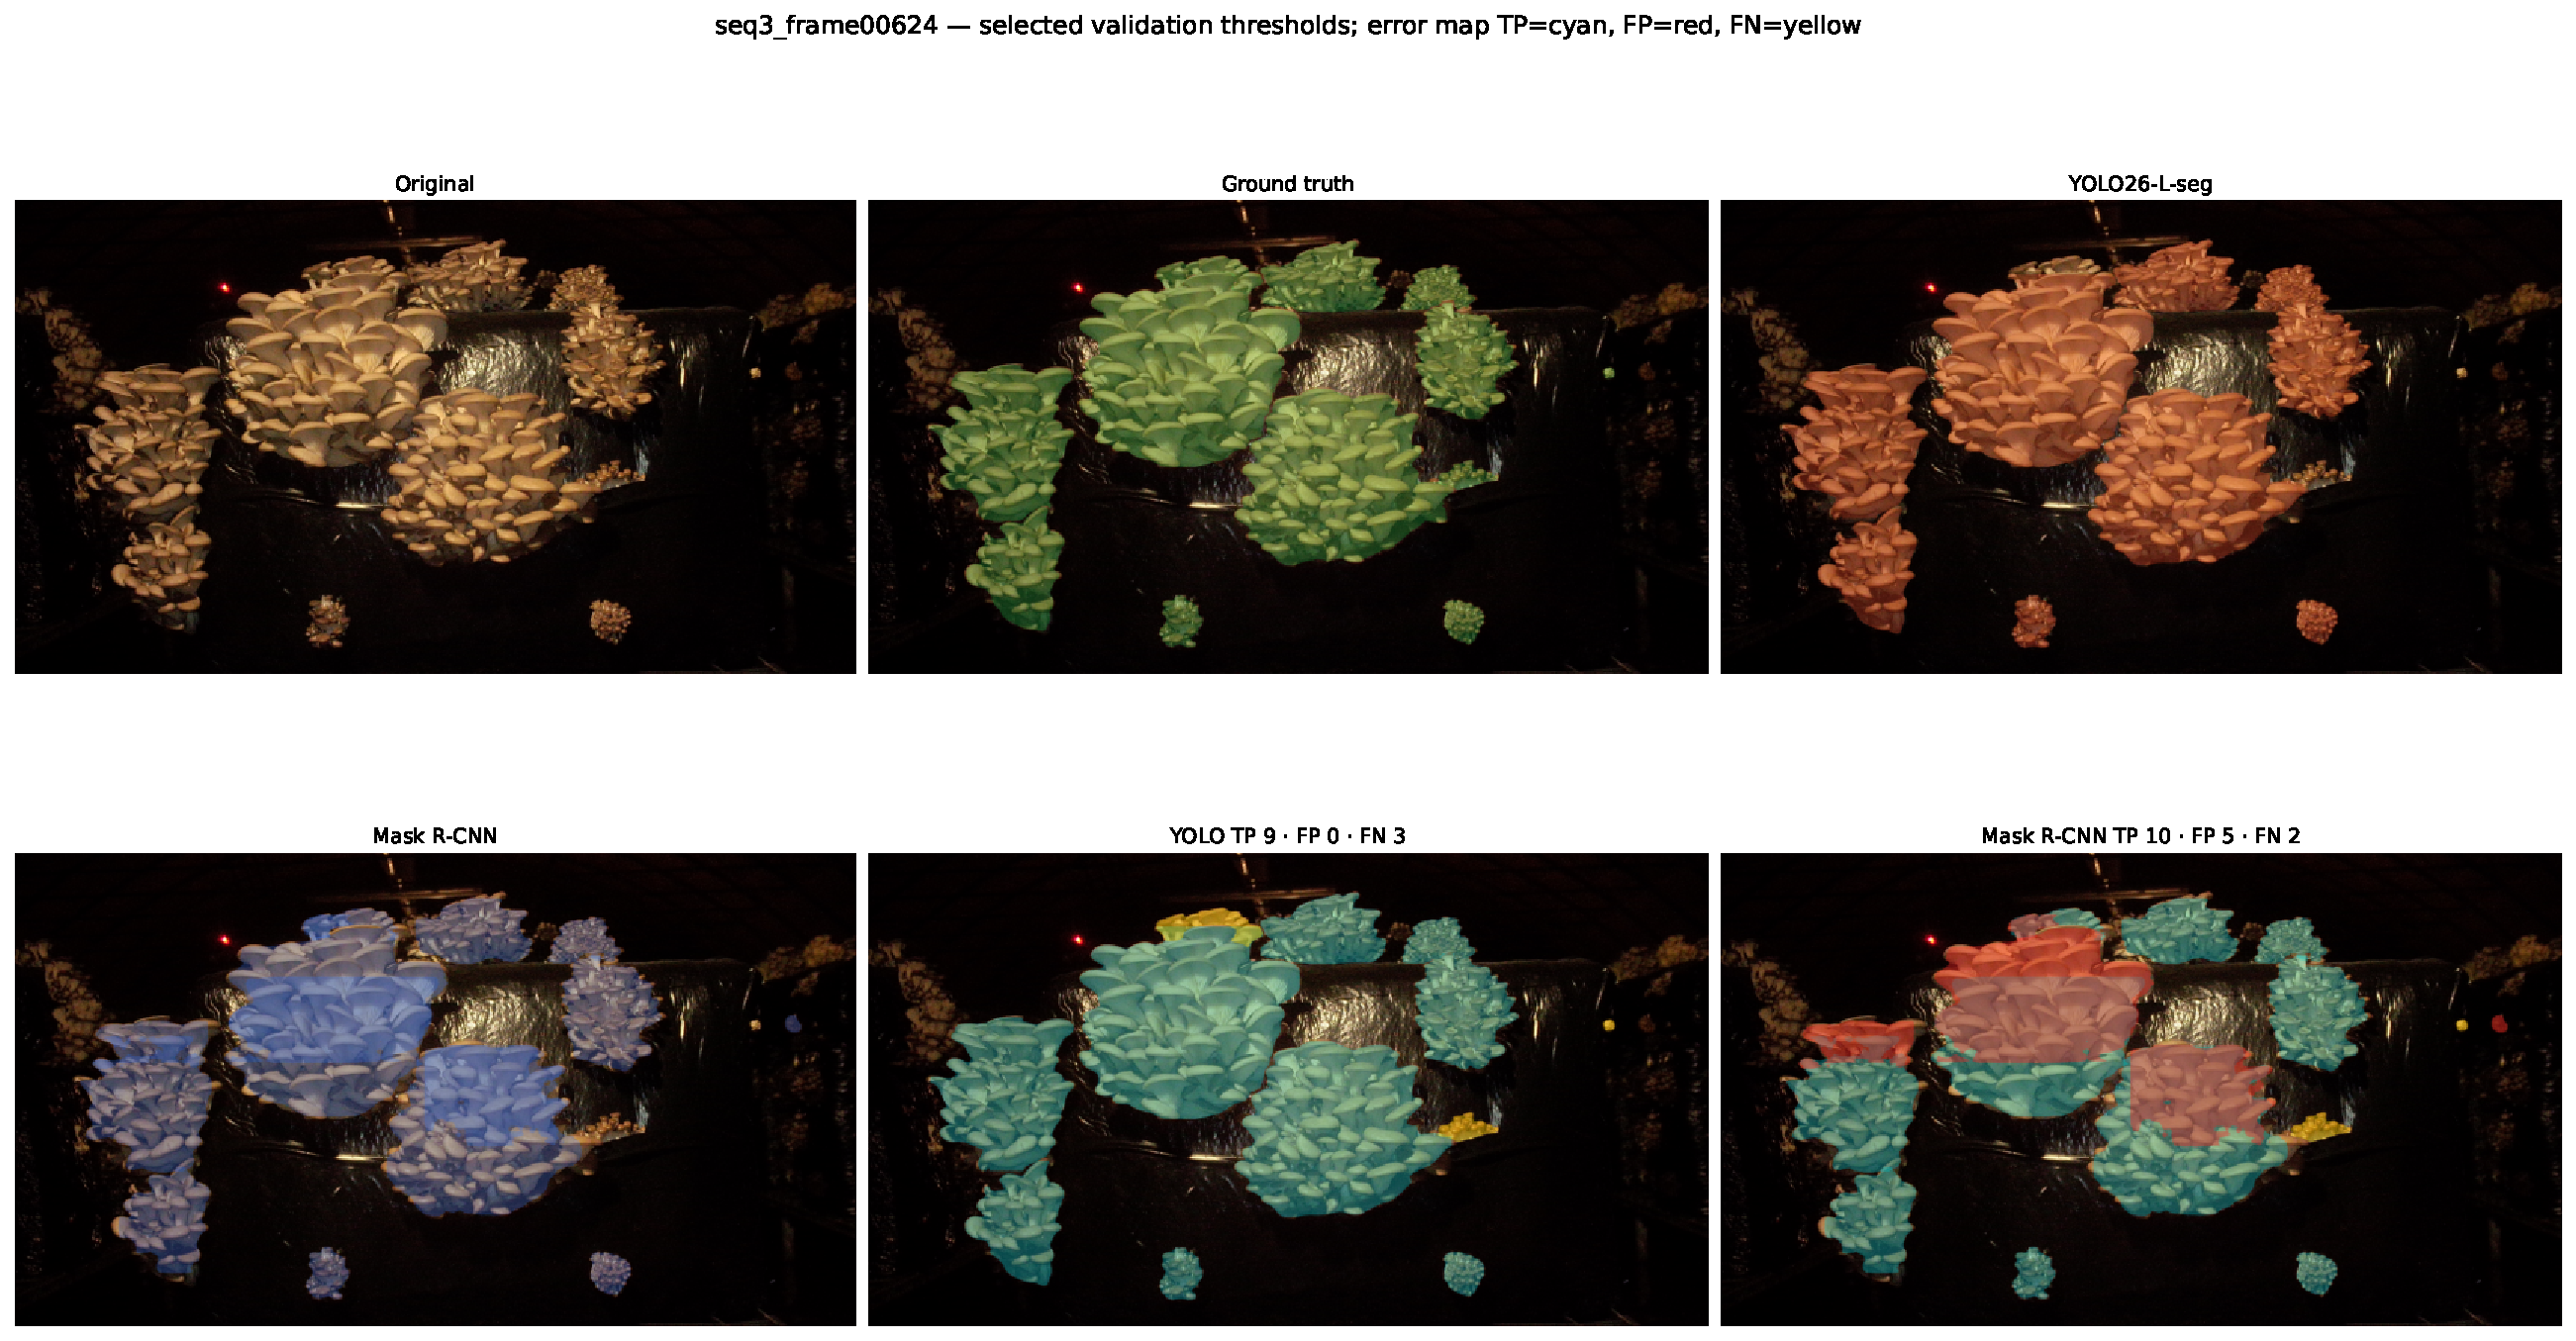
\includegraphics[width=0.76\linewidth]{figures/qualitative_hard_test.pdf}
\caption{Difficult test example (sequence 3, frame 624). The six panels show the original frame, source masks, both model predictions, and TP/FP/FN error maps. YOLO26-L-seg produced 9 TP, 0 FP, and 3 FN; Mask R-CNN produced 10 TP, 5 FP, and 2 FN at their respective validation-selected thresholds.}
\label{fig:qualitative-hard}
\end{figure}

\begin{figure}[H]
\centering
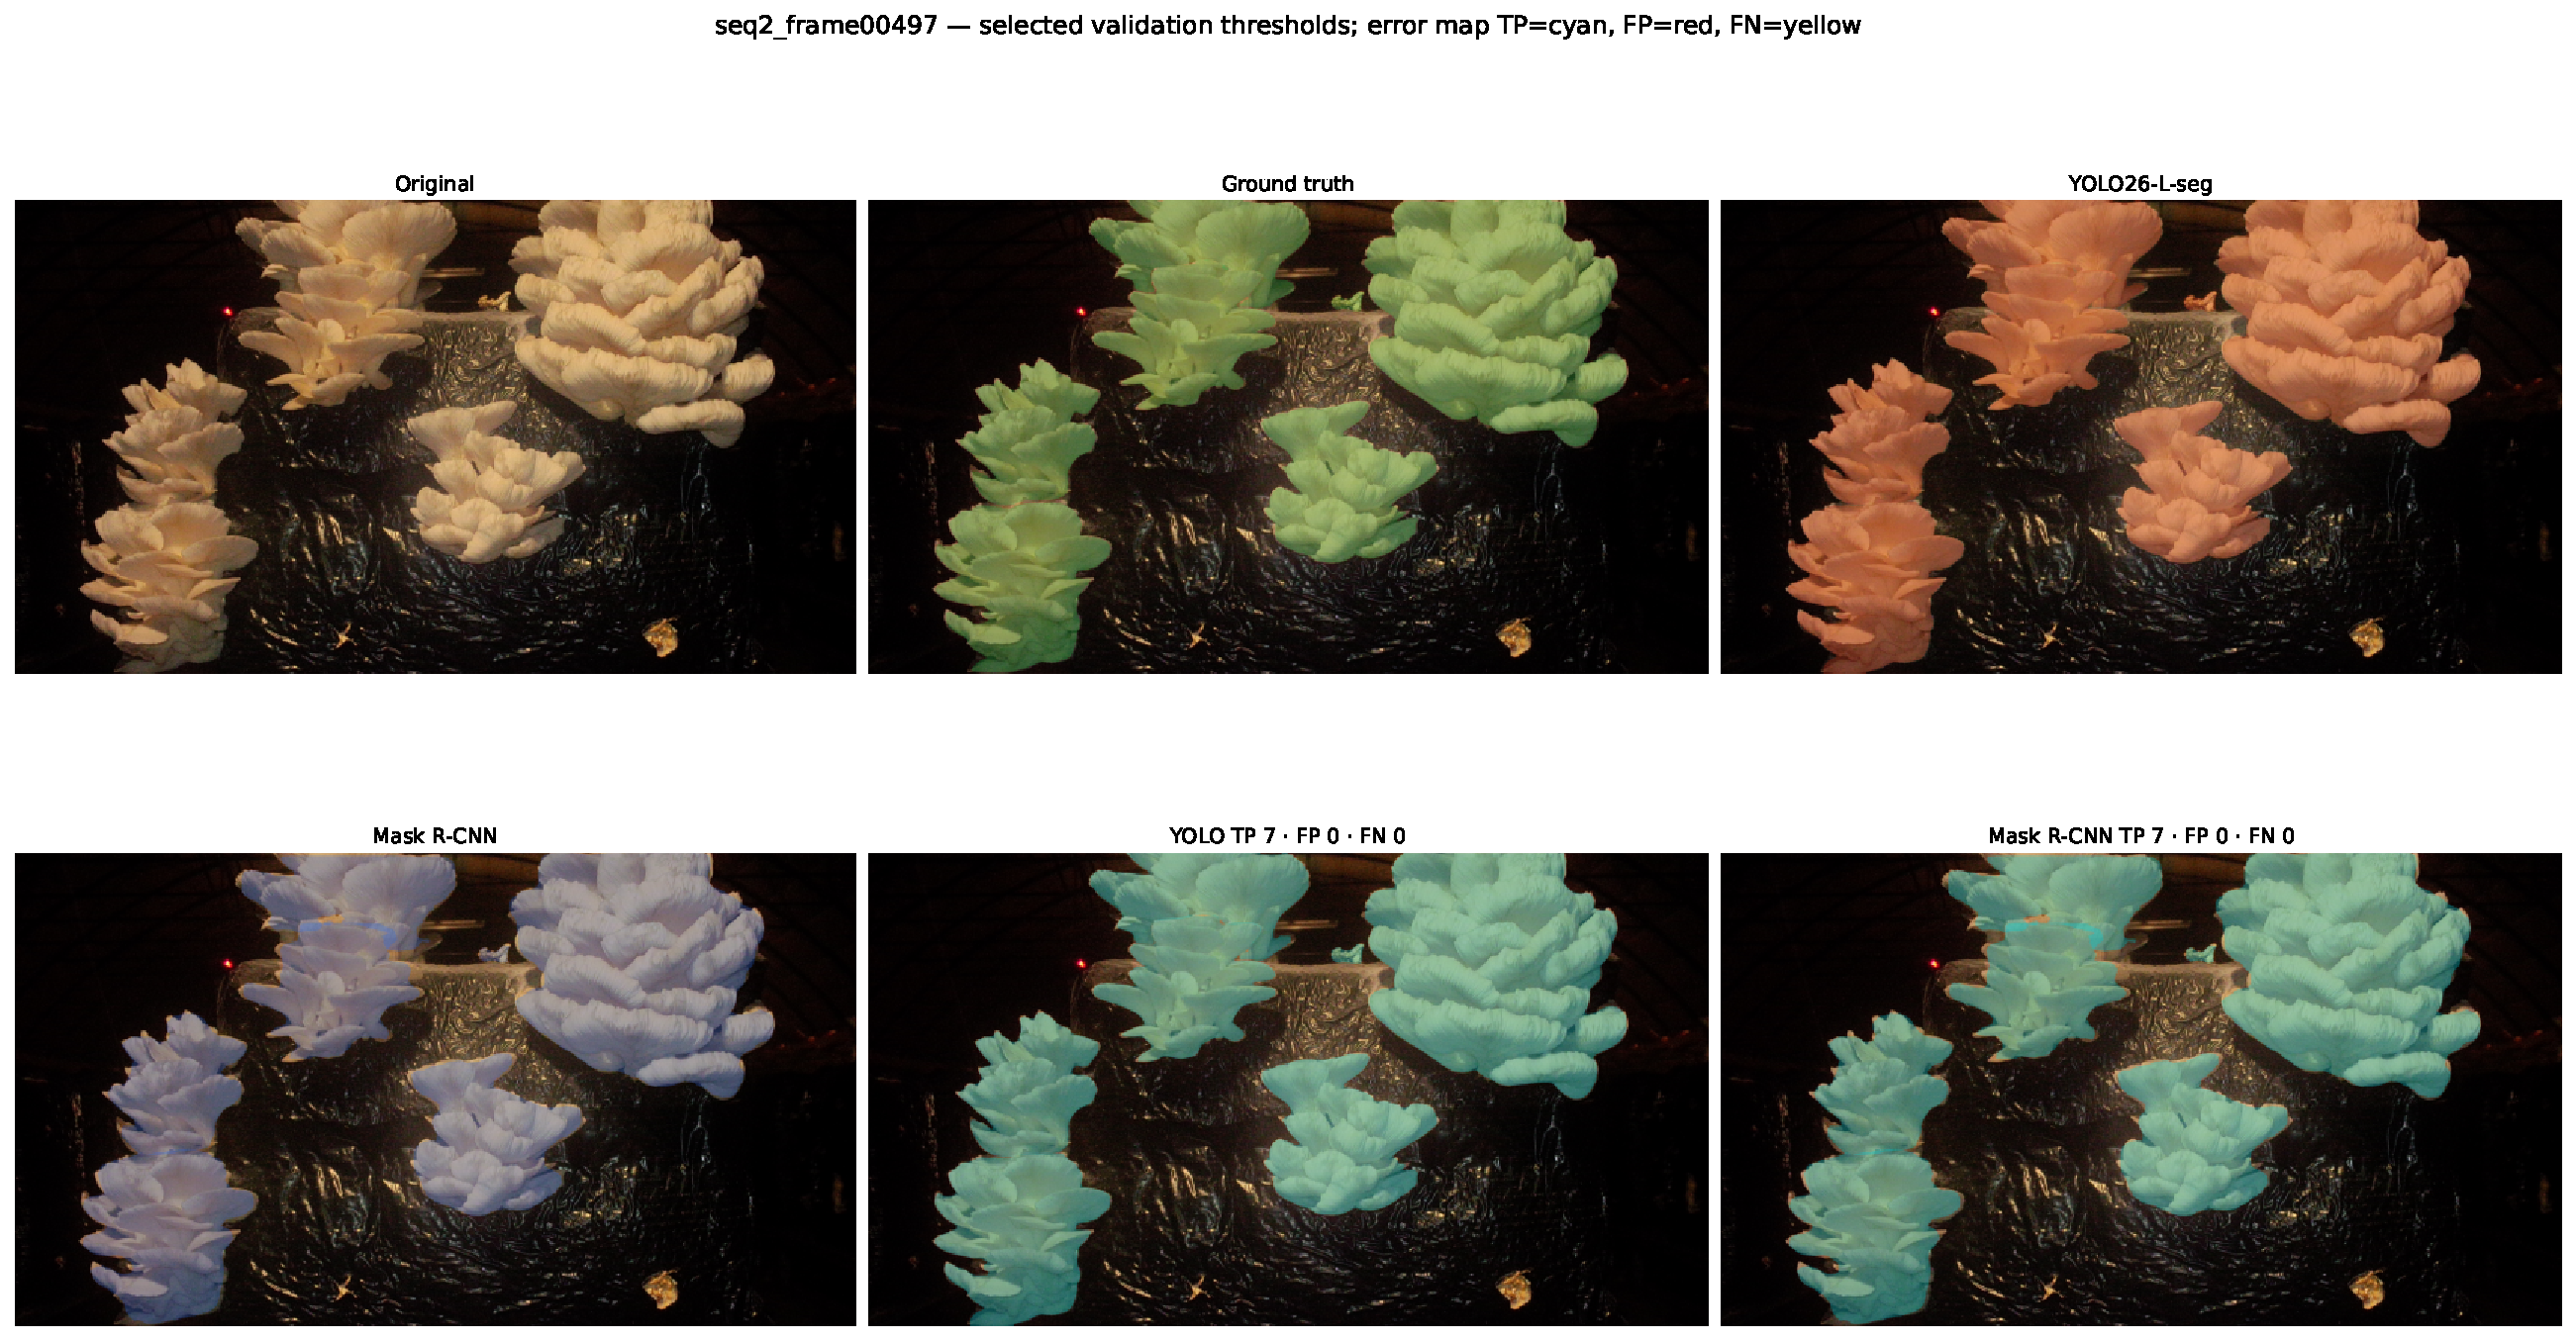
\includegraphics[width=0.76\linewidth]{figures/qualitative_clean_validation.pdf}
\caption{Clean validation example (sequence 2, frame 497). Both models matched the seven annotated clusters without false positives or missed instances at their respective selected thresholds.}
\label{fig:qualitative-clean}
\end{figure}
\FloatBarrier

\subsection{Per-Cluster Measurement Accuracy}

Segmentation quality matters here because mask errors propagate directly into area and bounding-box measurements. Predictions were matched one-to-one to ground-truth masks within each frame at IoU 0.50. For each measurement $m$ (area, width, or height), the mean relative absolute error is computed over the $N$ matched pairs as
\begin{equation}
\operatorname{RAE}_{m}=\frac{100}{N}\sum_{i=1}^{N}\frac{|\hat{m}_{i}-m_{i}|}{m_{i}},
\label{eq:rae}
\end{equation}
where $\hat{m}_{i}$ is the predicted value and $m_i$ is the corresponding ground-truth value. The table reports errors only for matched pairs; detection recall remains necessary to understand how many clusters were missed. YOLO26-L-seg had lower mean relative absolute error for all three measurements. Its area RAE was \textbf{4.21\%}, compared with 6.96\% for Mask R-CNN, while the width and height errors were also smaller.

\begin{table}[H]
\centering\small
\caption{Per-instance measurement errors on matched test instances. MAE is in image-space pixels or pixels squared; RAE is the mean per-instance relative absolute error.}
\label{tab:measurement}
\begin{tabular}{llrrr}
\toprule
Measurement & Model & Matched $n$ & MAE & RAE \\
\midrule
Area (px$^2$) & YOLO26-L-seg & 2,290 & \textbf{10,918.30} & \textbf{4.21\%} \\
Area (px$^2$) & Mask R-CNN & 2,479 & 33,286.18 & 6.96\% \\
Width (px) & YOLO26-L-seg & 2,290 & \textbf{9.46} & \textbf{1.49\%} \\
Width (px) & Mask R-CNN & 2,479 & 43.25 & 5.63\% \\
Height (px) & YOLO26-L-seg & 2,290 & \textbf{8.94} & \textbf{1.56\%} \\
Height (px) & Mask R-CNN & 2,479 & 47.67 & 7.42\% \\
\bottomrule
\end{tabular}
\end{table}

\begin{figure}[H]
\centering
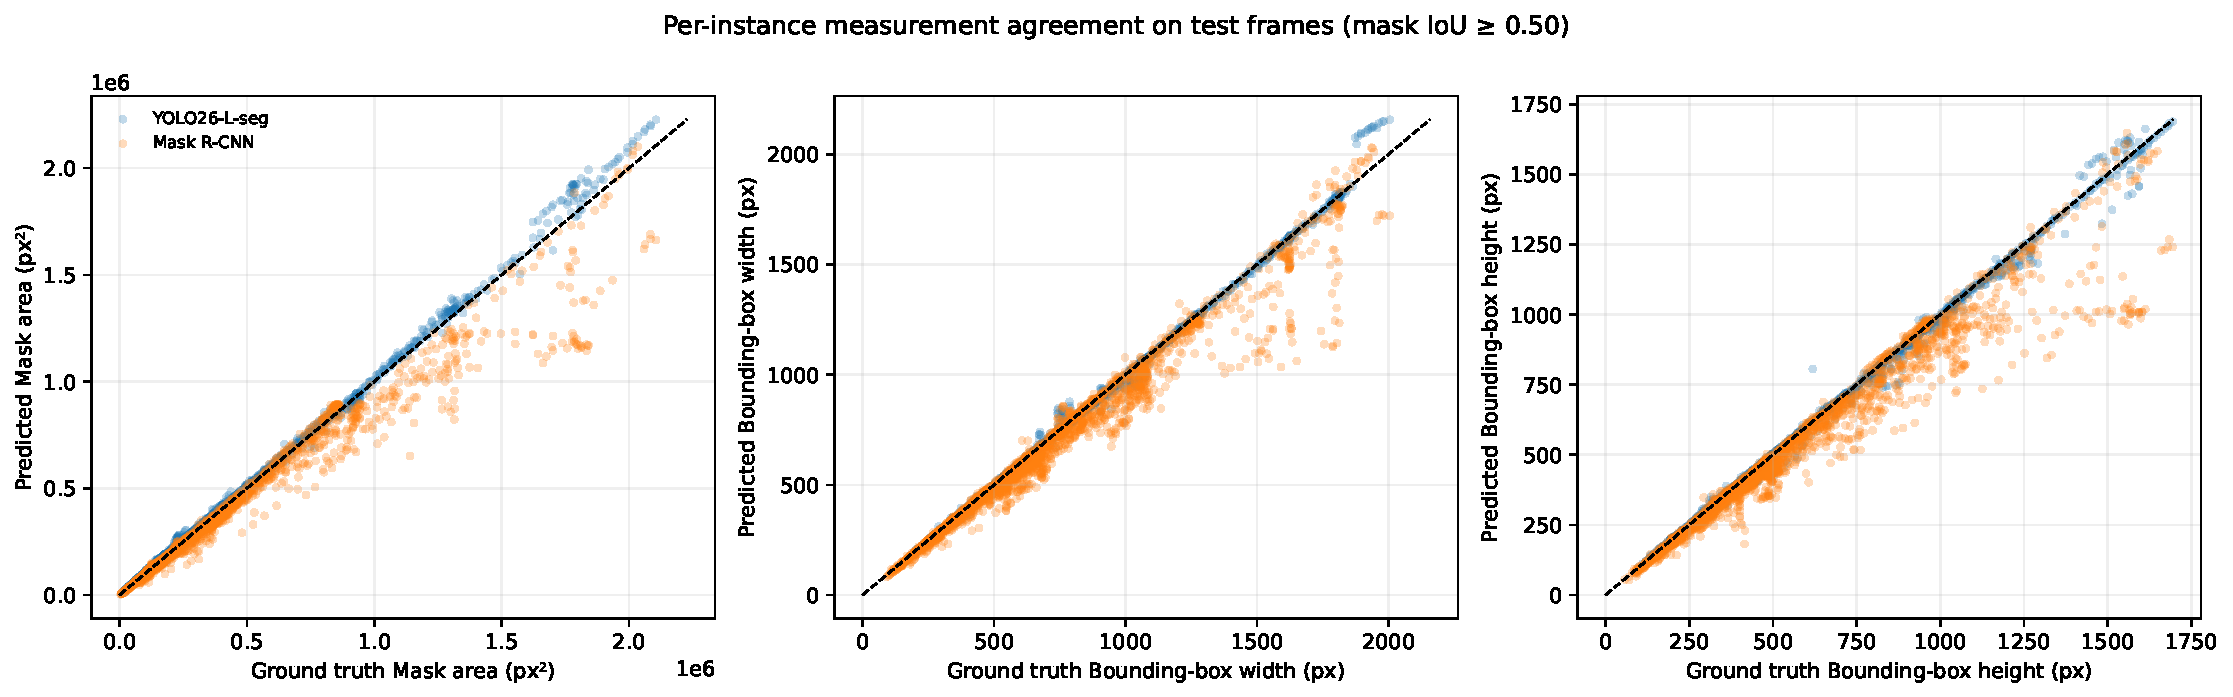
\includegraphics[width=0.95\linewidth]{figures/measurement_agreement.pdf}
\caption{Ground-truth versus predicted area, width, and height for matched test instances. The diagonal represents perfect agreement.}
\label{fig:measurement-agreement}
\end{figure}

\subsection{Temporal Tracking and Growth-History Monitoring}

The frozen tracker was evaluated on 528 test frames containing 2,663 annotated cluster observations. The low-confidence stage made 143 recovery assignments; this count does not mean that all 143 were true-positive matches. Under the frame-level evaluation threshold of mask IoU 0.50, 125 assignments matched previously unmatched ground-truth instances; the remaining 18 were unmatched and account for 18 of the 34 tracker false positives. The 2,290 matched instances reported for YOLO26-L-seg in Table~\ref{tab:measurement} are the high-confidence matches at the fixed validation-selected threshold. The tracker therefore adds 125 true positives through low-confidence recovery, giving 2,415 true positives overall (2,290 + 125). Performance was not uniform: sequence 3 had lower identity consistency and accounted for most missed observations and identity switches (Figure~\ref{fig:tracking-sequence}).

To distinguish reliable histories from identity merges, we assessed purity over each complete predicted track. A track was retained for strict growth analysis only when at least 90\% of its matched observations belonged to one dominant source identity. Of 28 predicted tracks with at least one ground-truth match, 27 passed and one failed. Five source identities were fragmented across multiple predicted tracks, and one identity had no strict history (Figure~\ref{fig:history-coverage}).

The rejected track occurred in sequence 3. Of its 246 matched observations, 154 belonged to the dominant source identity and 92 to a second identity, giving 62.60\% purity. The entire track was therefore excluded, rather than removing only the observations from the secondary identity (Figure~\ref{fig:mixed-purity}).

On the accepted histories, pooled RAE was \textbf{4.36\%} for area, \textbf{1.54\%} for width, and \textbf{1.65\%} for height. Temporal agreement was assessed between adjacent sampled observations within the same tracklet, without interpolation across missing observations. Across 2,140 eligible transitions, pooled and macro adjacent relative-area-change MAE were \textbf{1.52} and \textbf{1.76 percentage points}, respectively. Growth-direction agreement used the 5-percentage-point deadband defined in Eq.~\ref{eq:growth-direction-class}; macro agreement across 22 identities was \textbf{89.75\%}, with sequence-level agreement of 92.27\% for sequence 1 and 87.23\% for sequence 3 (Figures~\ref{fig:tracking-sequence} and~\ref{fig:adjacent-change}).

The geometric errors in Table~\ref{tab:growth-summary} use only source-consistent matches and therefore differ from the matched-instance population in Table~\ref{tab:measurement}.

\begin{table}[H]
\centering\small
\caption{Tracking and source-identity-aware growth-history results for the frozen tracker on the test sequences.}
\label{tab:growth-summary}
\begin{tabular}{lr}
\toprule
Measure & Result \\
\midrule
Test frames / GT observations & 528 / 2,663 \\
TP / FP / FN & 2,415 / 34 / 248 \\
MOTA / IDF1 & \textbf{89.19\% / 85.56\%} \\
Identity switches / fragmented source identities & 6 / 5 \\
Low-confidence recovery assignments (TP / FP) & 143 (125 / 18) \\
Ordinary matched observations & 2,415 (\textbf{90.69\% pooled}) \\
Strict source-consistent observations & \textbf{2,169 (81.45\% pooled)} \\
Macro strict history coverage & \textbf{82.45\%} \\
Purity-evaluable predicted tracks accepted / rejected & \textbf{27} / 1 \\
Strict area / width / height RAE (pooled) & \textbf{4.36\% / 1.54\% / 1.65\%} \\
Adjacent relative-area-change MAE (pooled / macro) & \textbf{1.52 / 1.76 pp} \\
Growth-direction agreement (macro) & \textbf{89.75\%} \\
Eligible adjacent transitions / identities & 2,140 / 22 \\
\bottomrule
\end{tabular}
\end{table}

\begin{figure}[H]
\centering
\begin{minipage}[t]{0.48\linewidth}
\centering
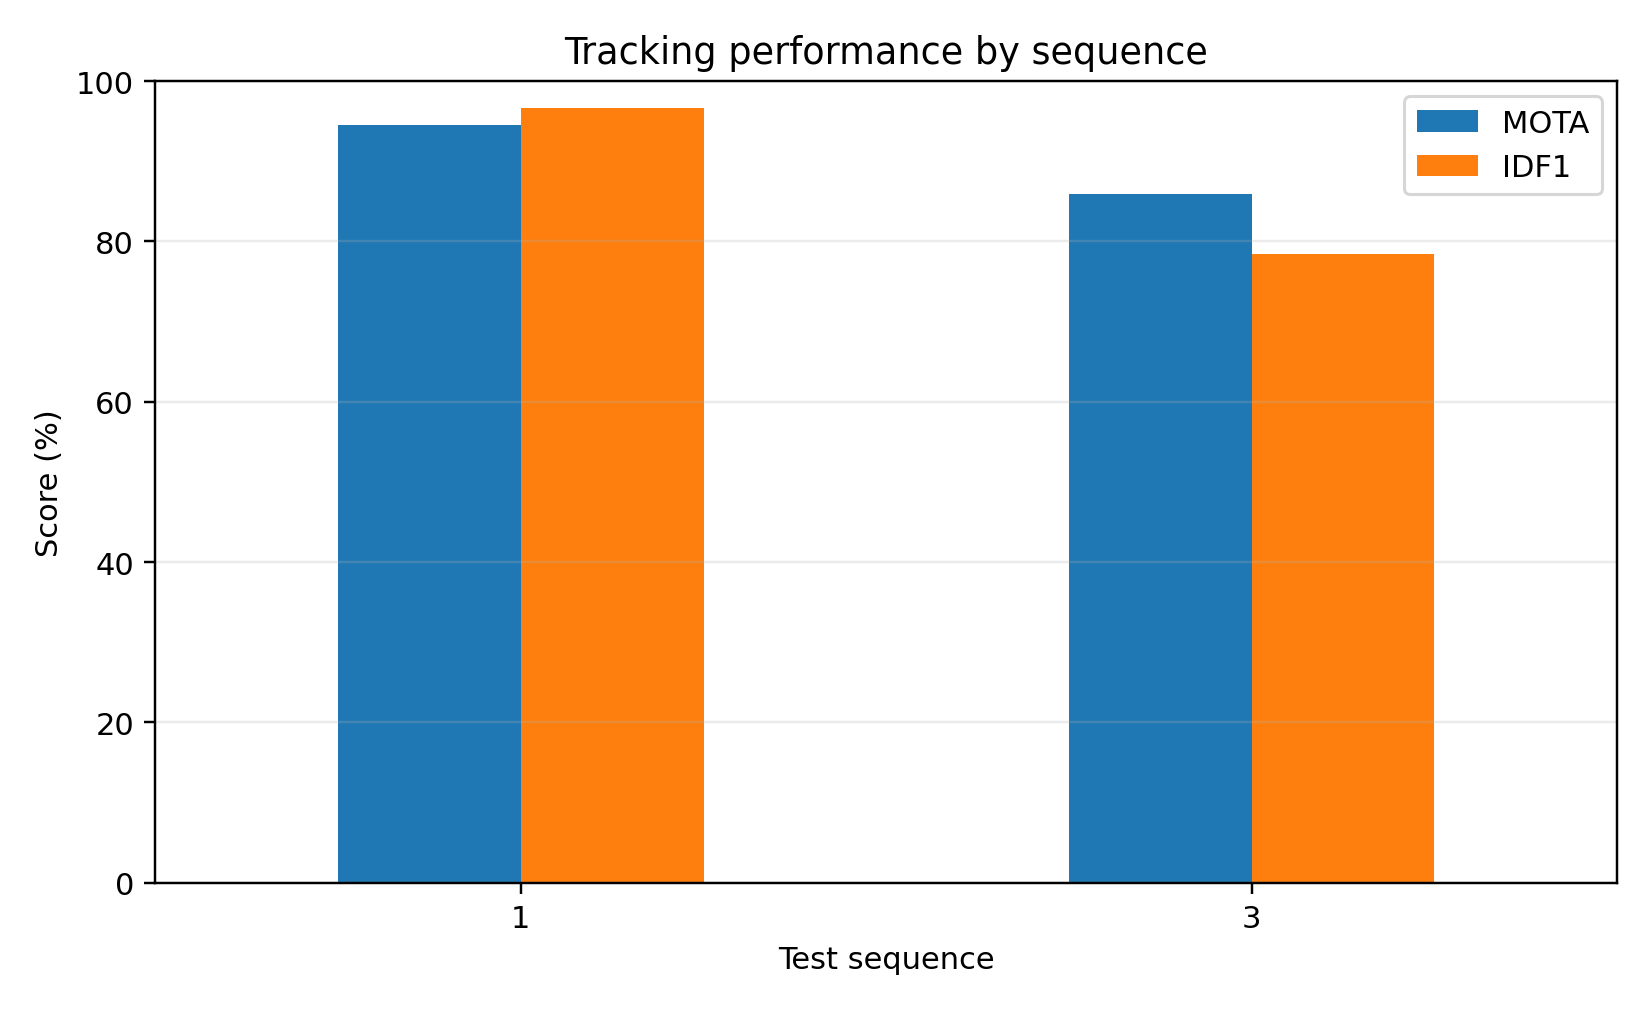
\includegraphics[width=\linewidth]{figures/fig_tracking_mota_idf1_by_sequence.png}
\par\small (a) MOTA and IDF1.
\end{minipage}\hfill
\begin{minipage}[t]{0.48\linewidth}
\centering
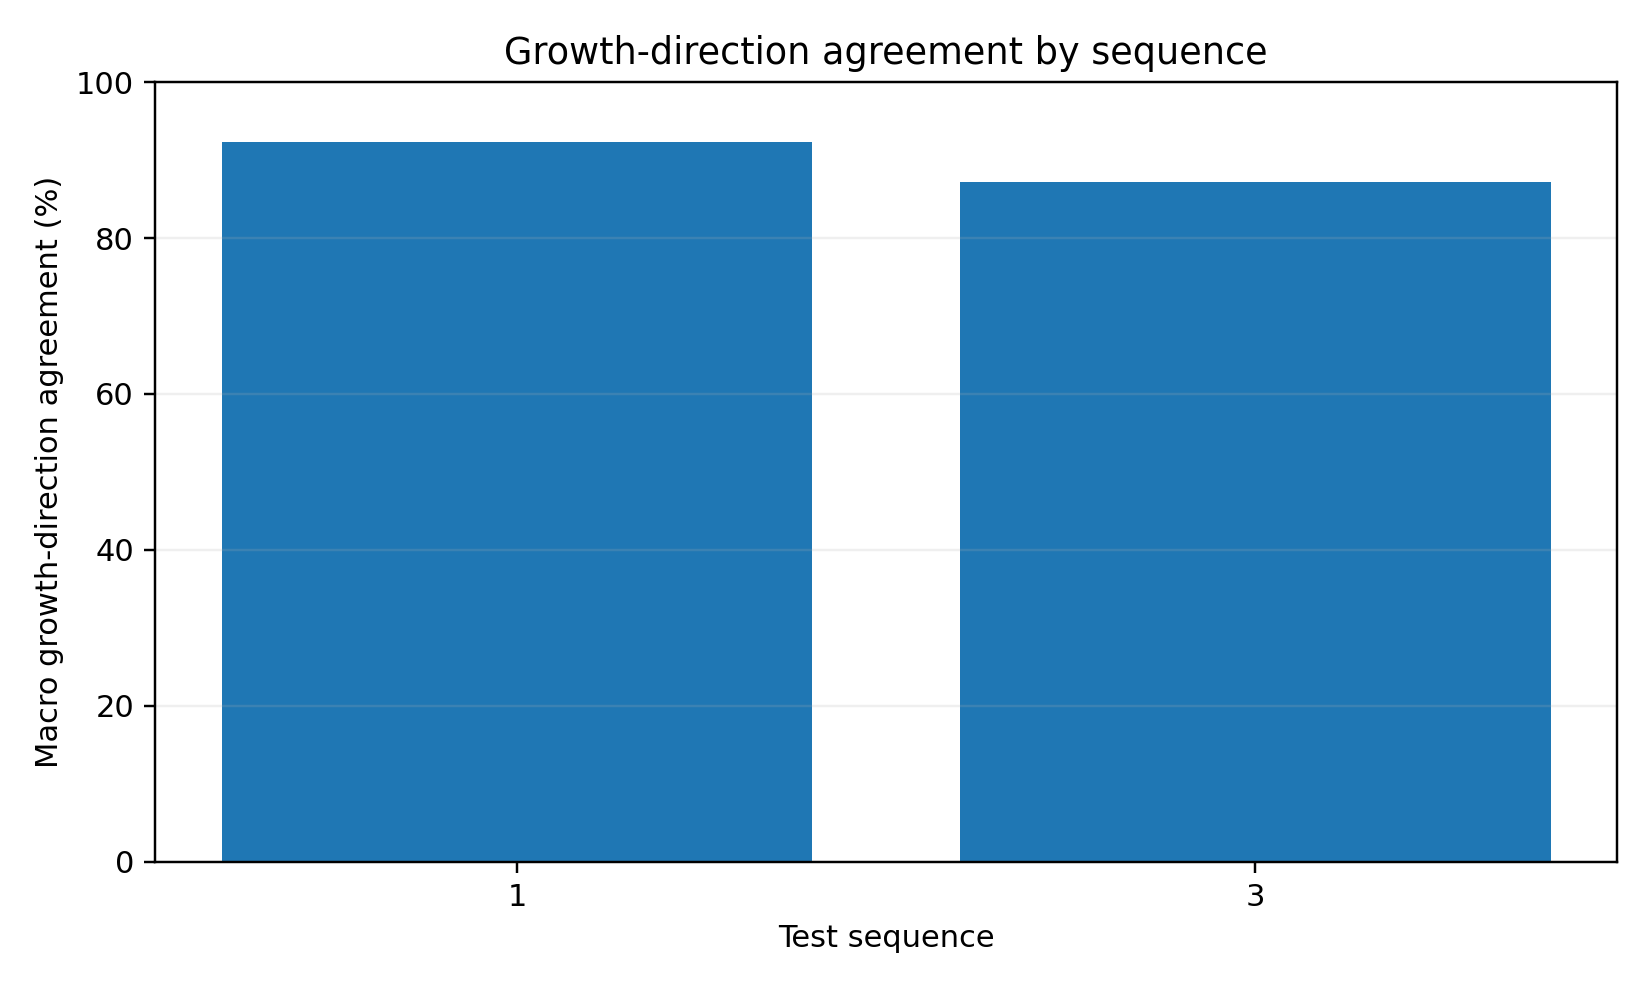
\includegraphics[width=\linewidth]{figures/fig_growth_direction_agreement.png}
\par\small (b) Growth-direction agreement.
\end{minipage}
\caption{Sequence-level tracking and growth-direction results. Sequence 3 has lower identity consistency and lower growth-direction agreement than sequence 1.}
\label{fig:tracking-sequence}
\end{figure}

\begin{figure}[H]
\centering
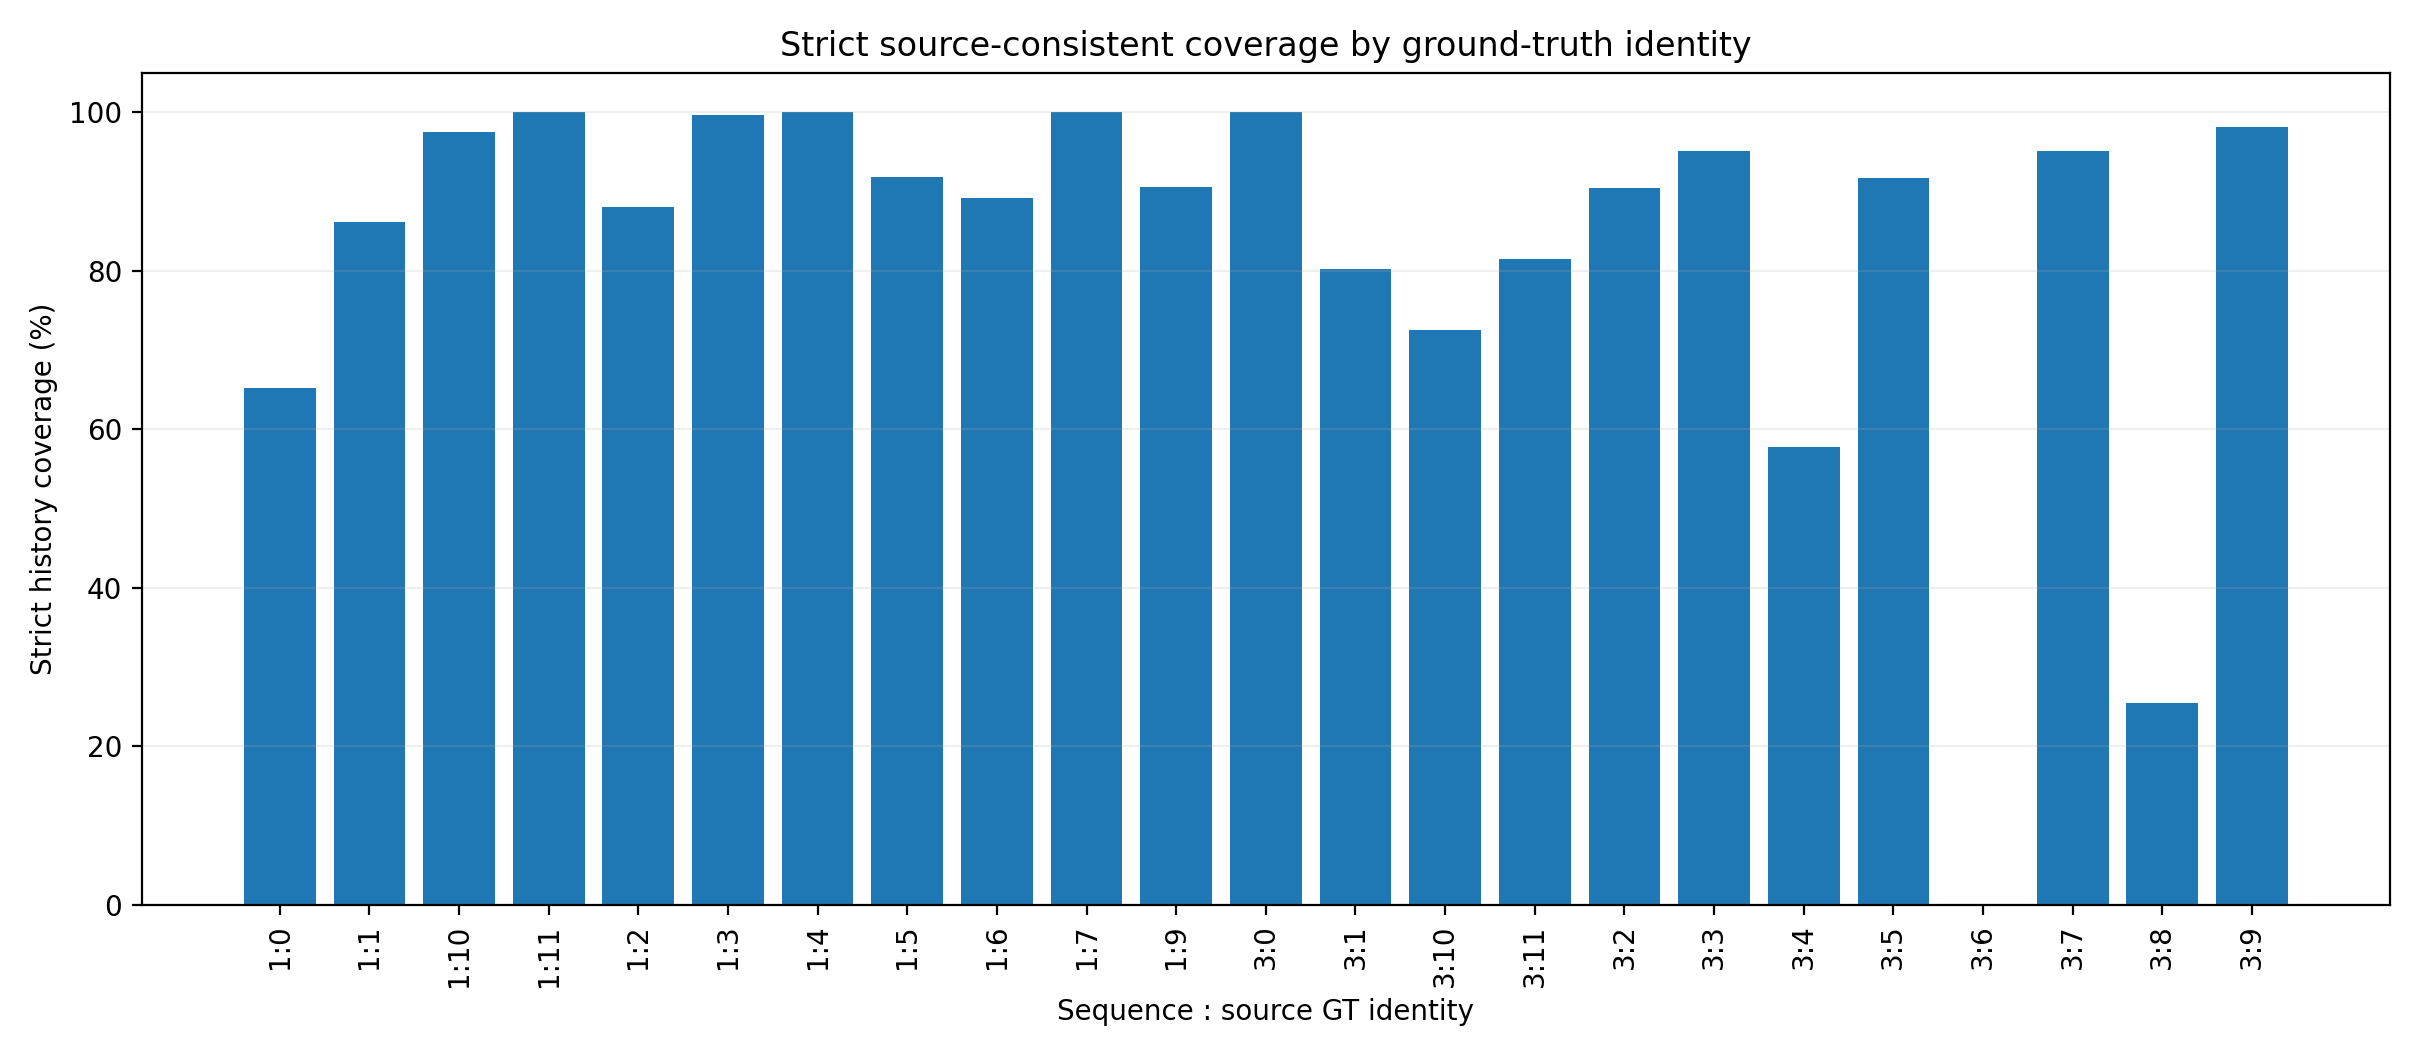
\includegraphics[width=0.98\linewidth]{figures/fig_strict_history_coverage_by_identity.png}
\caption{Strict source-consistent observation coverage for each ground-truth identity. The 90\% criterion is applied to complete predicted-track purity before per-identity coverage is calculated; it is not a threshold on the bars in this figure. The horizontal axis labels identify the sequence and source tracking ID.}
\label{fig:history-coverage}
\end{figure}

\begin{figure}[H]
\centering
\begin{minipage}[t]{0.58\linewidth}
\centering
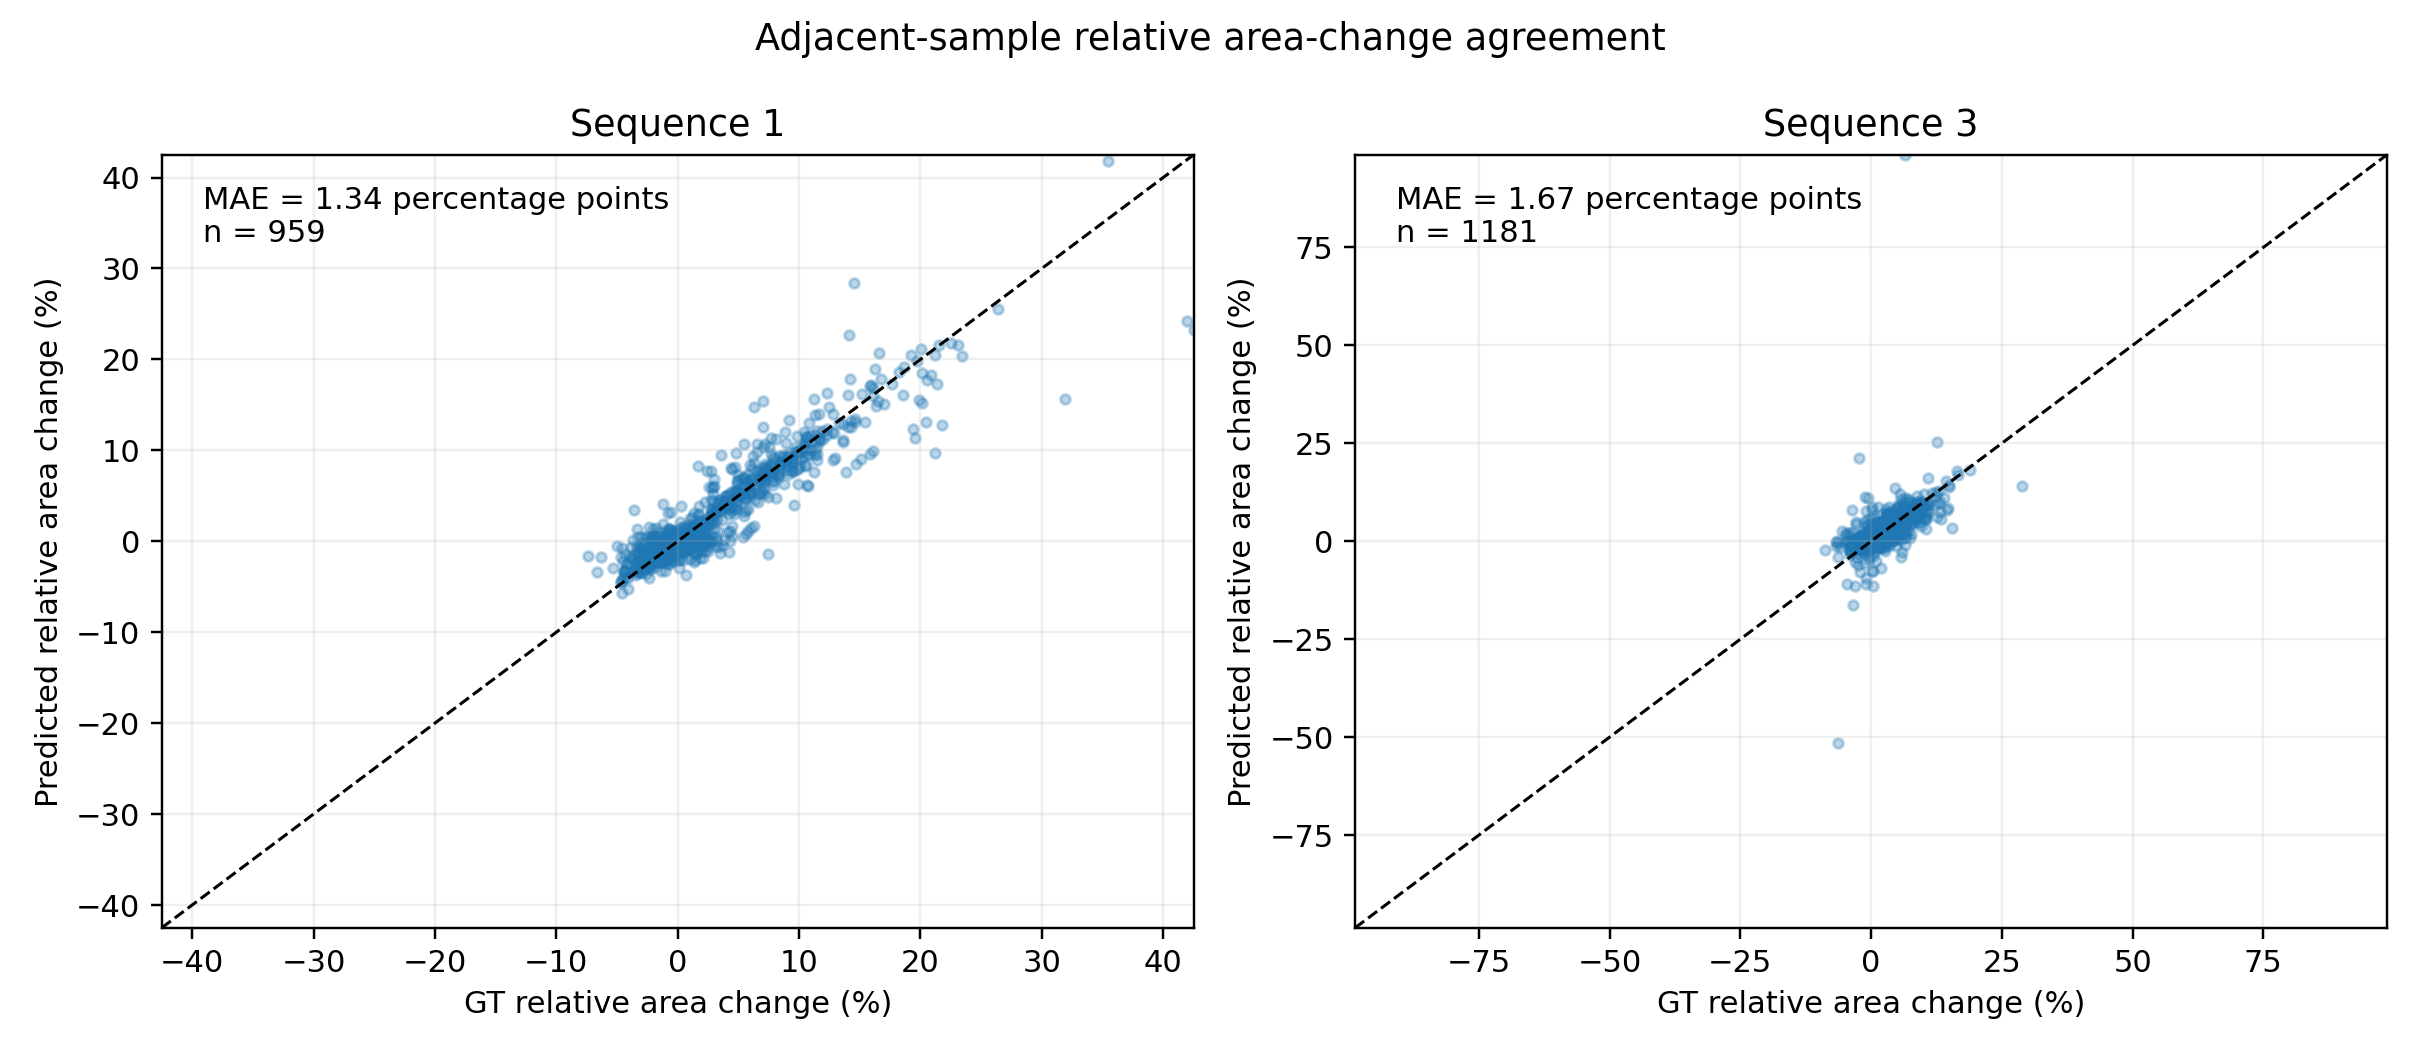
\includegraphics[width=\linewidth]{figures/fig_adjacent_relative_area_change_agreement.png}
\par\small (a) Predicted versus annotated relative area change.
\end{minipage}\hfill
\begin{minipage}[t]{0.38\linewidth}
\centering
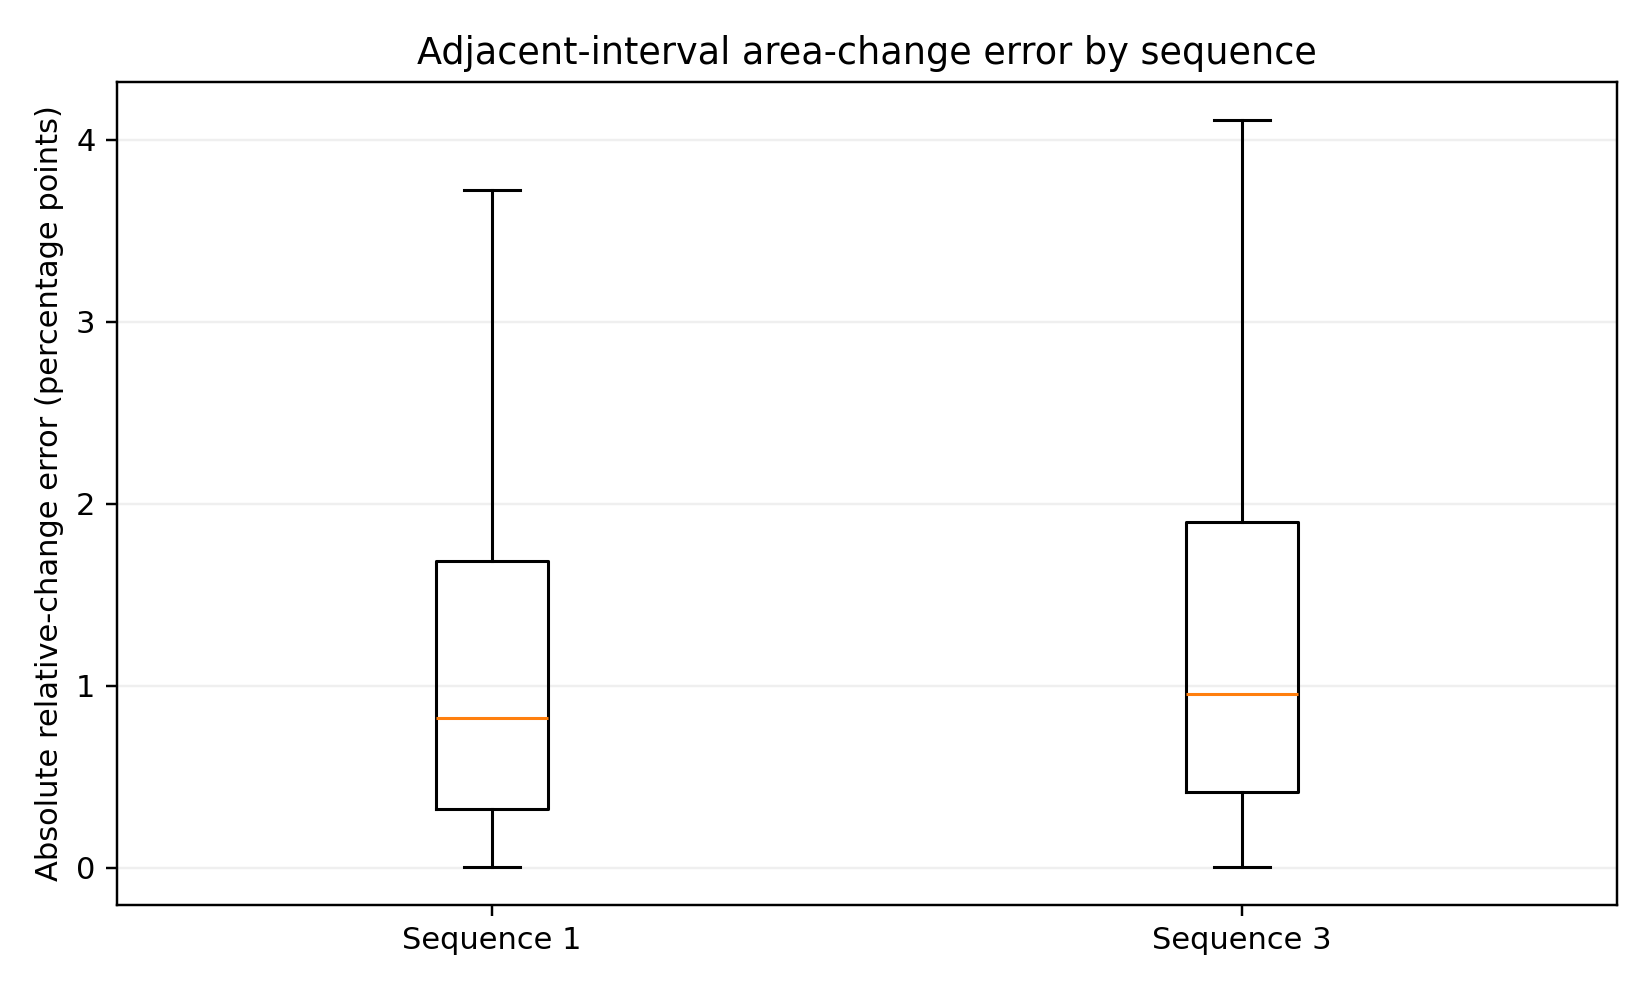
\includegraphics[width=\linewidth]{figures/fig_adjacent_area_change_error_by_sequence.png}
\par\small (b) Absolute change error by sequence.
\end{minipage}
\caption{Agreement in relative area change between consecutive sampled observations within accepted tracklets. The scatter panels show the relation between predicted and annotated changes; the box plots summarize absolute error in percentage points.}
\label{fig:adjacent-change}
\end{figure}

\begin{figure}[H]
\centering
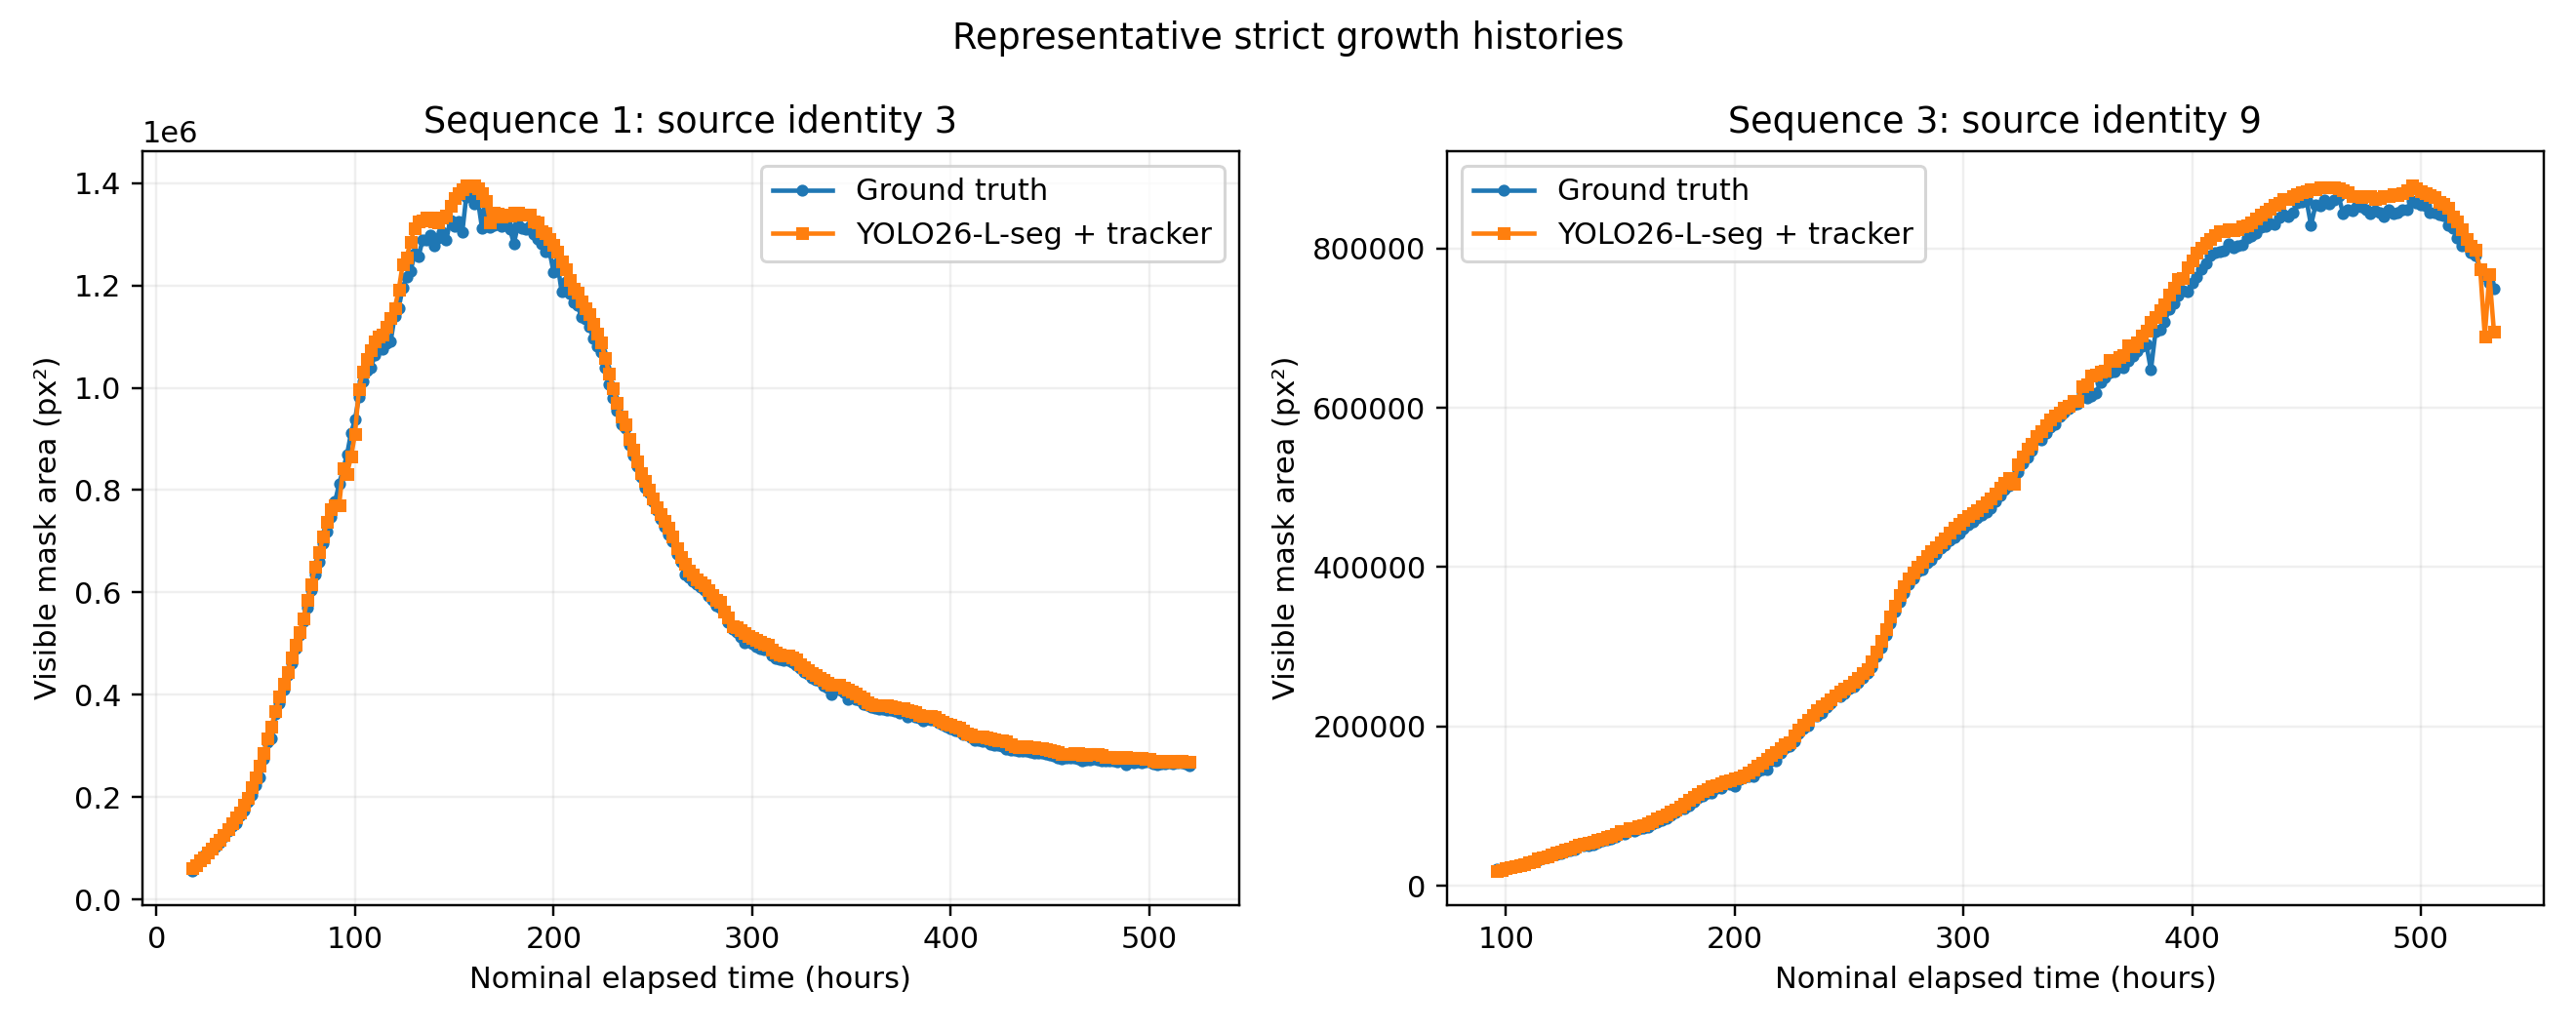
\includegraphics[width=0.95\linewidth]{figures/fig_representative_growth_trajectories.png}
\caption{Representative source-consistent area histories from test sequences 1 and 3. Predicted and annotated mask areas are shown over nominal elapsed time; the examples illustrate accepted histories and are not intended to represent every cluster.}
\label{fig:representative-trajectories}
\end{figure}

% Keep the two supporting figures in the same reading sequence, immediately
% after the representative growth histories; do not force a new page here.
\begin{figure}[H]
\centering
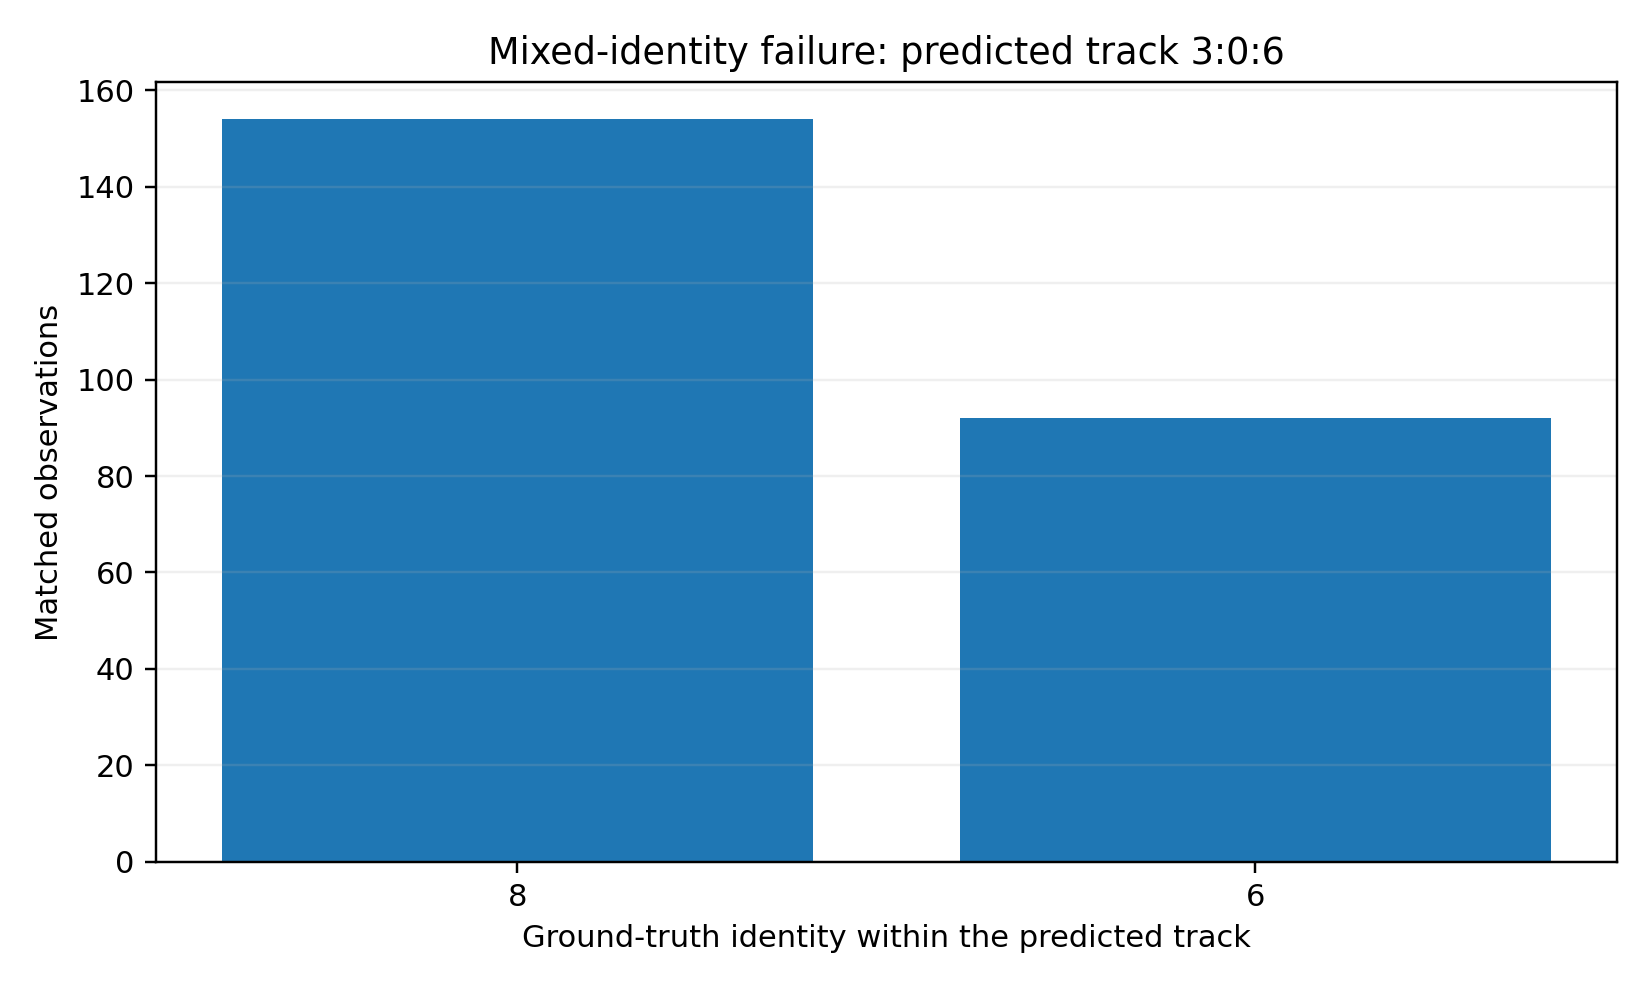
\includegraphics[width=0.52\linewidth]{figures/fig_mixed_identity_track_failure.png}
\caption{Composition of the mixed-identity predicted track in sequence 3. Of 246 matched observations, 154 (62.60\%) belong to the dominant source identity and 92 (37.40\%) to a second identity; the complete track is excluded by the 90\% purity rule.}
\label{fig:mixed-purity}
\end{figure}
\vspace{-0.35em}
\begin{figure}[H]
\centering
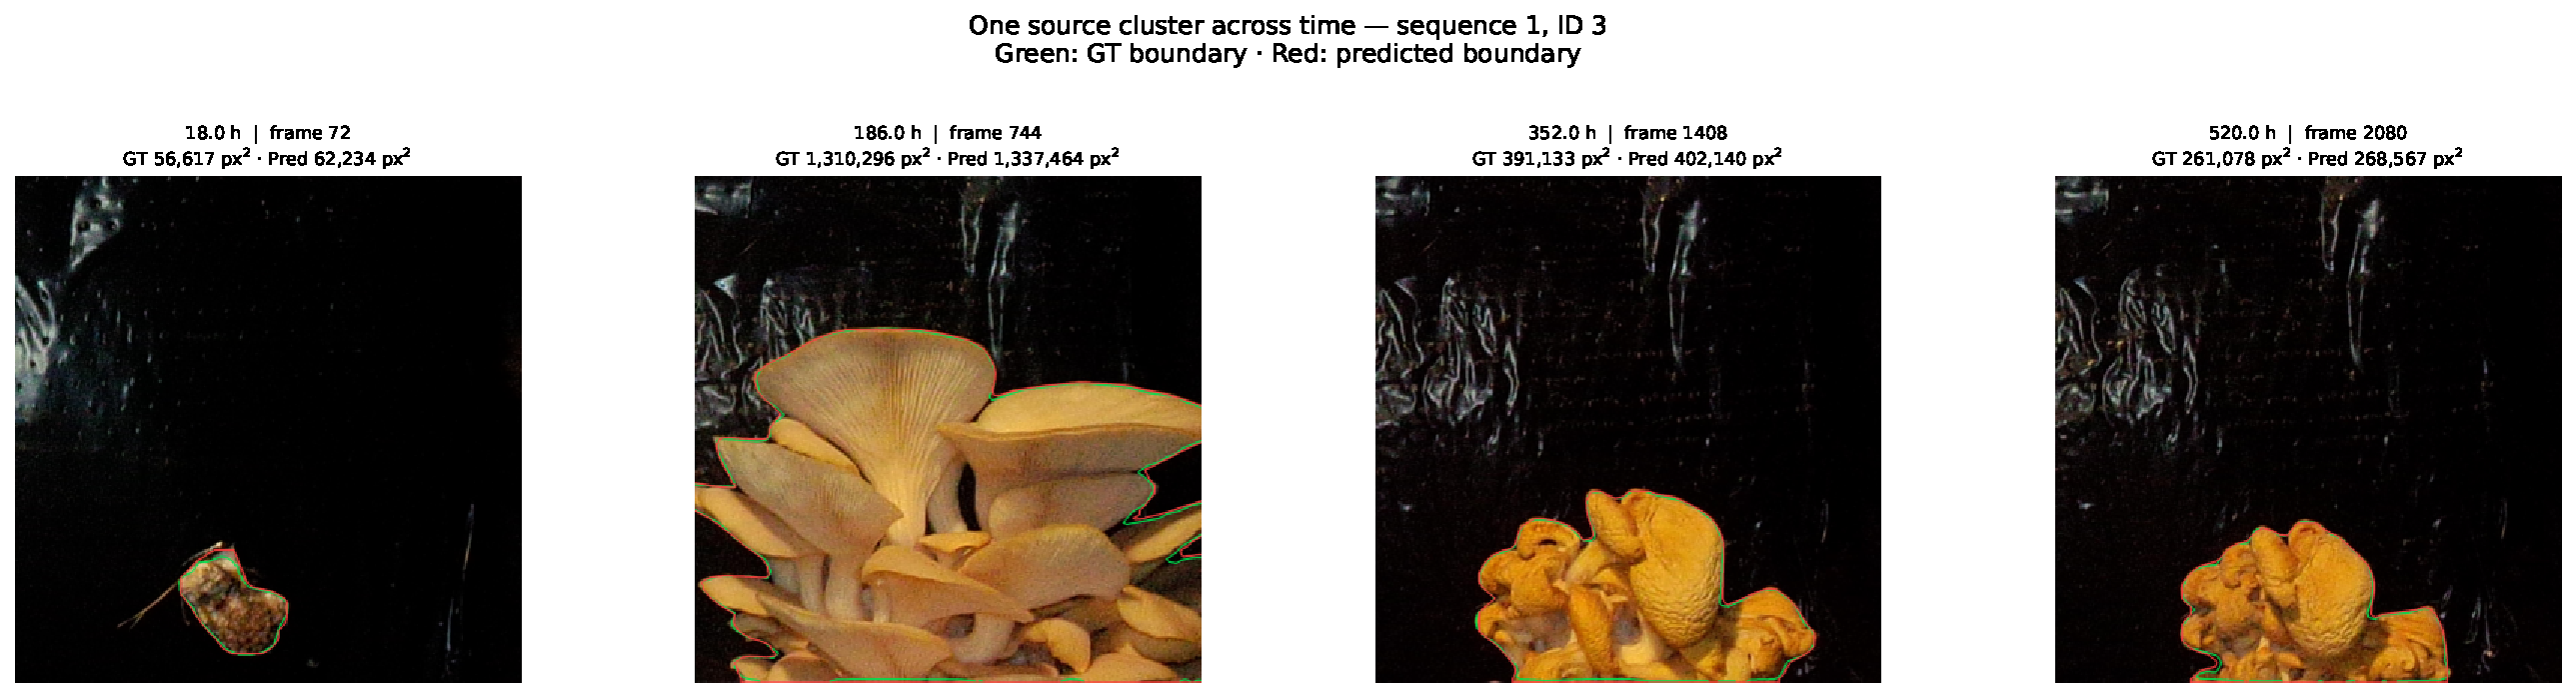
\includegraphics[width=0.95\linewidth]{figures/cluster_progression.pdf}
\caption{Four chronological observations of sequence 1, source identity 3. Green and red outlines denote the source mask and predicted mask, respectively. The selected observations are not consecutive; their nominal elapsed times are shown above each crop.}
\label{fig:cluster-progression}
\end{figure}
\vspace{0.35em}

\subsection{Comparison with Charisis et al.}

The two systems address the same cluster-level monitoring problem, but their tracking components make different assumptions. Charisis et al. first apply domain-specific filtering: they remove predictions below 0.20 confidence, suppress overlapping predictions at mask IoU 0.30, and use the substrate and previous cluster baselines to identify background, occluded, and post-harvest residual regions. Their association stage selects the highest-IoU current prediction for each stored cluster baseline and accepts it above 0.20. An unmatched baseline is retained across subsequent timesteps, allowing a temporarily missed or occluded cluster to be associated again when it reappears. Their sizing stage uses the known substrate dimensions (50 by 36 cm) as a reference for relative width and height estimates \cite{charisis}.

By contrast, the proposed pipeline performs global one-to-one assignment between active tracks and current YOLO26-L-seg masks using the last observed mask and a 0.10 association threshold. Its low-confidence stage can update an existing track, but the selected zero-gap policy closes a track after a missed sampled observation. The present implementation does not reproduce Charisis et al.'s substrate, background, duplicate, and post-harvest filtering, and it reports area, width, and height in pixels or pixels squared without physical-scale calibration. The main implementation differences are summarized in Table~\ref{tab:charisis-method-comparison}.

Both studies use the MOTA equation $1-(FP+FN+IDSW)/GT$, but this is not a controlled comparison. Charisis et al. report 96.7\% and 92.7\% on their first and third timelapse test sets; the proposed pipeline obtains 94.58\% and 85.87\% on source sequences 1 and 3 (Table~\ref{tab:mota-charisis}). Although both studies use the same source dataset, the present study evaluates every eighth frame, whereas Charisis reports results from its own segmentation and filtering pipeline. The evaluated frames, predictions, filtering, association, and matching therefore differ. The published values provide context, not evidence of direct superiority or equivalence.

\begin{table}[H]
\centering\scriptsize
\caption{Selected methodological differences between Charisis et al. and the proposed pipeline.}
\label{tab:charisis-method-comparison}
\begin{tabularx}{\linewidth}{p{2.4cm}XX}
\toprule
Component & Charisis et al. (2025) & Present study \\
\midrule
Segmentation & Mask R-CNN with ConvNeXt or Swin backbones; three maturity classes. & YOLO26-L-seg; one class, \texttt{mushroom\_cluster}. \\
Pre-association filtering & Confidence and duplicate suppression plus substrate-aware background, occlusion, and post-harvest residual filters. & Confidence thresholding and recovery; no equivalent substrate- or harvest-specific filter stage. \\
Association & Highest mask-IoU prediction for each stored baseline; threshold 0.20. & Global one-to-one assignment using the last observed mask; threshold 0.10. \\
Missed observations & Unmatched cluster baselines are retained for later reassociation. & Maximum gap zero; a track is closed after a missed sampled observation. \\
Growth sizing & Pixel-to-relative-size approximation using the known substrate dimensions. & Mask area and bounding-box width/height in image pixels; no physical calibration. \\
\bottomrule
\end{tabularx}
\end{table}

\begin{table}[H]
\centering\small
\caption{Contextual comparison of sequence-level MOTA. Charisis values are the published results for the first and third timelapse test sets; values for the present study use its own evaluation protocol.}
\label{tab:mota-charisis}
\begin{tabular}{lrrr}
\toprule
Timelapse / sequence & GT observations (present study) & MOTA (present study) & Charisis MOTA \\
\midrule
First / sequence 1 & 1,014 & 94.58\% & 96.70\% \\
Third / sequence 3 & 1,649 & 85.87\% & 92.70\% \\
\bottomrule
\end{tabular}
\end{table}
\FloatBarrier

\subsection{Runtime and Memory}

Both segmentation models were evaluated on an NVIDIA Tesla T4. Table~\ref{tab:runtime} summarizes model inference and mask-export times and peak host memory. The timers have different boundaries: the YOLO timer includes the synchronized Ultralytics prediction call, while the Mask R-CNN timer covers its model forward and ROI/box post-processing; the mask-export stages also perform different work. Across the combined inference run, peak CUDA allocation was 1.03 GiB and peak reserved memory was 1.25 GiB. The separate cached tracking evaluation processed 528 frames in 2.40 s (4.54 ms per frame); this excludes model inference. These measurements describe the recorded implementation and should not be interpreted as a controlled end-to-end speed ranking.

\begin{table}[H]
\centering\small
\caption{Runtime and memory measurements from the fresh Tesla T4 evaluation. Timing boundaries differ by model.}
\label{tab:runtime}
\resizebox{\linewidth}{!}{%
\begin{tabular}{lrrrr}
\toprule
Model & Inference mean (ms) & Inference p95 (ms) & Mask export mean (ms) & Peak host RSS (MiB) \\
\midrule
YOLO26-L-seg & 156.09 & 161.14 & 1,258.92 & 2,551.86 \\
Mask R-CNN + ConvNeXt & 344.41 & 386.10 & 5,085.54 & 2,627.89 \\
\bottomrule
\end{tabular}%
}
\end{table}

\section{Discussion}

The segmentation comparison favors YOLO26-L-seg on the available checkpoints. Its advantage is not limited to mask AP: the lower area, width, and height errors show that the difference carries through to measurements on matched instances. Mask R-CNN has higher recall at its selected threshold, but its lower precision reflects a larger number of false positives. These results support YOLO26-L-seg as the stronger checkpoint for this class-agnostic evaluation, not as a universal replacement for Mask R-CNN.

The tracking results show a larger difference between the two test sequences than the aggregate values alone suggest. Sequence 1 has relatively high MOTA and IDF1, while sequence 3 contributes most of the missed observations and identity errors. This uneven performance is also reflected in growth monitoring: the tracker preserves several long, useful histories, but fragmentation and one mixed-identity track reduce the number of observations that can be used with strict source consistency. The 90\% purity filter is therefore important not because it improves the tracker, but because it prevents an incorrect identity merge from being interpreted as a single cluster's growth.

The contextual Charisis comparison suggests that substrate-aware filtering and persistence across missed observations are important differences between the systems. The present results do not isolate the effect of either design choice, but the lower sequence-3 scores and the mixed-identity failure identify missed-detection handling and cluster separation as priorities for further study. Because the evaluated frame subsets and full pipelines differ, the published MOTA values should not be interpreted as a controlled performance ranking.

The adjacent relative-area-change results add a temporal view beyond per-instance geometric error. The predicted changes remain close to annotated changes for many transitions, but the larger spread in sequence 3 and its lower growth-direction agreement show that reliable segmentation and identity matching do not guarantee equally reliable growth trajectories. These measurements describe visible image-space changes; they do not establish physical growth rates or biological maturity.

\subsection{Error Analysis}

The principal identity error is the mixed predicted track in sequence 3, which combines observations from two source identities. Fragmentation creates the opposite failure: one source cluster is divided across several predicted tracks, shortening its usable history. Detection misses also reduce coverage even when the remaining matches retain the correct identity. The qualitative segmentation examples show that frame-level mask quality varies, while the tracking and growth-history results show how these errors propagate through time.

\subsection{Limitations}

The evaluation uses one species and four time-lapse sequences from one published dataset. Although test frames were held out from model training, the test sequences were inspected during tracker development; the reported tracking results are retrospective. MOTA uses the equation reported by Charisis et al. with the project's own one-to-one frame matching at mask IoU 0.50 and its stated identity-switch accounting; it is not a reproduction of their full tracking pipeline or a TrackEval implementation. The Mask R-CNN checkpoint is a TorchVision adaptation rather than the original MMDetection model.

Test frames are sampled every two hours, although the source camera captured images every fifteen minutes. The selected tracker closes a track after a missed sampled observation and therefore cannot bridge longer gaps. Raw capture timestamps were unavailable, so growth plots use nominal time. Measurements remain two-dimensional pixel area and bounding-box dimensions; no physical calibration, volume, mass, or harvest-readiness estimate is claimed. The relative-size index is a reference to the training mean area of the source \texttt{well-defined} category, not a maturity classifier.

\subsection{Future Work}

The most direct improvement is to evaluate identity persistence across missed observations on a new, untouched cultivation sequence, with any gap policy selected using validation data. Broader testing across cultivation rooms, camera positions, and mushroom batches is also needed. A verified substrate reference and camera calibration could support physical-size estimates, while biological maturity prediction would require explicit validation against expert labels and fruitbody characteristics rather than size alone.

\Needspace{8\baselineskip}
\section{Conclusions}

This study evaluated instance segmentation and cluster-level growth monitoring on a four-sequence oyster mushroom time-lapse dataset. YOLO26-L-seg achieved higher mask AP than the available Mask R-CNN--ConvNeXt baseline and lower matched-instance errors for area, width, and height. Its frozen mask-IoU tracker obtained \textbf{89.19\% MOTA} and \textbf{85.56\% IDF1} on the 528 test frames. Under a 90\% whole-track purity rule, 2,169 of 2,663 annotated observations were retained for source-consistent growth histories, giving \textbf{82.45\% macro coverage}. Across 2,140 eligible adjacent transitions, macro growth-direction agreement was \textbf{89.75\%}, and pooled adjacent relative-area-change MAE was \textbf{1.52 percentage points}. The results support mask-based image-space growth monitoring, while showing that identity continuity, missed detections, and sequence-dependent performance remain important limitations.

\begingroup\small
\begin{thebibliography}{00}
\setlength{\itemsep}{0.12em}
\bibitem{charisis} C. Charisis, S. Nuwayhid, and D. Argyropoulos, ``A novel Mask R-CNN-based tracking pipeline for oyster mushroom cluster growth monitoring in time-lapse image datasets,'' \emph{Computers and Electronics in Agriculture}, vol. 237, Part A, Art. no. 110590, 2025, doi: 10.1016/j.compag.2025.110590.
\bibitem{otsu} N. Otsu, ``A threshold selection method from gray-level histograms,'' \emph{IEEE Trans. Systems, Man, and Cybernetics}, vol. 9, no. 1, pp. 62--66, 1979, doi: 10.1109/TSMC.1979.4310076.
\bibitem{watershed} L. Vincent and P. Soille, ``Watersheds in digital spaces: An efficient algorithm based on immersion simulations,'' \emph{IEEE Trans. Pattern Analysis and Machine Intelligence}, vol. 13, no. 6, pp. 583--598, 1991, doi: 10.1109/34.87344.
\bibitem{maskrcnn} K. He, G. Gkioxari, P. Doll\'ar, and R. Girshick, ``Mask R-CNN,'' in \emph{Proc. IEEE Int. Conf. Computer Vision (ICCV)}, 2017, pp. 2961--2969, doi: 10.1109/ICCV.2017.322.
\bibitem{convnext} Z. Liu, H. Mao, C.-Y. Wu, C. Feichtenhofer, T. Darrell, and S. Xie, ``A ConvNet for the 2020s,'' in \emph{Proc. IEEE/CVF Conf. Computer Vision and Pattern Recognition (CVPR)}, 2022, pp. 11976--11986, doi: 10.1109/CVPR52688.2022.01167.
\bibitem{yolo26docs} Ultralytics, ``YOLO26,'' Ultralytics Documentation. [Online]. Available: \url{https://docs.ultralytics.com/models/yolo26}. Accessed: Nov. 23, 2026.
\bibitem{dataset} C. Charisis, S. Nuwayhid, and D. Argyropoulos, ``Oyster mushroom clusters growth monitoring timelapses,'' Zenodo, 2025, doi: 10.5281/zenodo.15041243.
\bibitem{pytorch} A. Paszke et al., ``PyTorch: An imperative style, high-performance deep learning library,'' in \emph{Advances in Neural Information Processing Systems}, vol. 32, pp. 8026--8037, 2019.
\bibitem{torchvision} TorchVision maintainers and contributors, ``TorchVision: PyTorch's Computer Vision library,'' GitHub repository, released Nov. 6, 2016. [Online]. Available: \url{https://github.com/pytorch/vision}. Accessed: Nov. 23, 2026.
\bibitem{scipy} P. Virtanen et al., ``SciPy 1.0: Fundamental algorithms for scientific computing in Python,'' \emph{Nature Methods}, vol. 17, pp. 261--272, 2020, doi: 10.1038/s41592-019-0686-2.
\bibitem{crouse} D. F. Crouse, ``On implementing 2D rectangular assignment algorithms,'' \emph{IEEE Trans. Aerospace and Electronic Systems}, vol. 52, no. 4, pp. 1679--1696, 2016, doi: 10.1109/TAES.2016.140952.
\bibitem{coco} T.-Y. Lin et al., ``Microsoft COCO: Common Objects in Context,'' in \emph{Proc. European Conf. Computer Vision (ECCV)}, 2014, pp. 740--755, doi: 10.1007/978-3-319-10602-1\_48.
\bibitem{opencv} G. Bradski, ``The OpenCV Library,'' \emph{Dr. Dobb's Journal of Software Tools}, 2000.
\end{thebibliography}
\endgroup

\appendix
\begingroup\small
\setlength{\parskip}{0.12em}
\section{How to Run the Code}

The project repository is available at \url{https://github.com/h-nam-sys/Oyster-Mushroom-Cluster-Monitoring}. The workflow uses two complementary notebooks. \texttt{full-inference.ipynb} performs model inference and exports the cached prediction and provenance bundle. \texttt{tracking-and-growth-history.ipynb} consumes that bundle to evaluate temporal association, source-identity consistency, and growth histories; it does not repeat segmentation inference. In Kaggle, attach the \href{https://www.kaggle.com/datasets/hnamedu/fungicirno-models}{Oyster Mushroom Cluster Monitoring Models dataset}, which provides the selected YOLO26-L-seg and Mask R-CNN checkpoints and canonical split manifest, and obtain the original four-sequence image dataset separately from the Charisis Zenodo record (\url{https://doi.org/10.5281/zenodo.15041243}). The source images are not redistributed with this report or repository.

For fresh inference, select a Kaggle GPU accelerator, open \texttt{full-inference.ipynb}, and run all cells from top to bottom. It searches recursively under \texttt{/kaggle/input} and \texttt{/kaggle/working} for model artifacts, the split manifest, and source sequences; the source archives can also be retrieved through the notebook's configured Drive fallback when they are not attached. It verifies the manifest and checkpoint hashes, performs inference on all 961 validation and test frames, and packages the predictions, segmentation metrics, figures, provenance records, and integrity report. For the downstream evaluation, attach the resulting evidence bundle and run \texttt{tracking-and-growth-history.ipynb}. That notebook verifies the cached prediction records and frozen tracker configuration, then exports tracking and growth-history metrics, figures, and an integrity report without rerunning either segmentation model.

The recorded inference environment used Python 3.13.16, PyTorch 2.11.0+cu130, TorchVision 0.26.0+cu130, CUDA 13.0, Ultralytics 8.4.214, NumPy 2.1.3, pandas 2.3.3, and OpenCV 4.14.0 \cite{opencv} on an NVIDIA Tesla T4. The inference settings and memory-safe CPU mask-pasting procedure are described in the Methodology section. The tracking evaluation uses the same cached YOLO predictions and SciPy assignment implementation; its runtime is reported separately from model inference.

\section{Declaration of AI Tool Usage}

The team used ChatGPT (OpenAI, GPT-6) for technical discussion, code and notebook development/debugging, review and interpretation of experiment artifacts, and restructuring and editing of the report. ChatGPT did not perform the reported model training or inference. The team executed the experiments, reviewed the generated outputs, and is responsible for the methods, results, figures, and final submitted text.

\endgroup
\end{document}
